% Options for packages loaded elsewhere
\PassOptionsToPackage{unicode}{hyperref}
\PassOptionsToPackage{hyphens}{url}
%
\documentclass[
]{book}
\usepackage{amsmath,amssymb}
\usepackage{lmodern}
\usepackage{iftex}
\ifPDFTeX
  \usepackage[T1]{fontenc}
  \usepackage[utf8]{inputenc}
  \usepackage{textcomp} % provide euro and other symbols
\else % if luatex or xetex
  \usepackage{unicode-math}
  \defaultfontfeatures{Scale=MatchLowercase}
  \defaultfontfeatures[\rmfamily]{Ligatures=TeX,Scale=1}
\fi
% Use upquote if available, for straight quotes in verbatim environments
\IfFileExists{upquote.sty}{\usepackage{upquote}}{}
\IfFileExists{microtype.sty}{% use microtype if available
  \usepackage[]{microtype}
  \UseMicrotypeSet[protrusion]{basicmath} % disable protrusion for tt fonts
}{}
\makeatletter
\@ifundefined{KOMAClassName}{% if non-KOMA class
  \IfFileExists{parskip.sty}{%
    \usepackage{parskip}
  }{% else
    \setlength{\parindent}{0pt}
    \setlength{\parskip}{6pt plus 2pt minus 1pt}}
}{% if KOMA class
  \KOMAoptions{parskip=half}}
\makeatother
\usepackage{xcolor}
\IfFileExists{xurl.sty}{\usepackage{xurl}}{} % add URL line breaks if available
\IfFileExists{bookmark.sty}{\usepackage{bookmark}}{\usepackage{hyperref}}
\hypersetup{
  pdftitle={データ解析},
  pdfauthor={水圏植物生態学研究室},
  hidelinks,
  pdfcreator={LaTeX via pandoc}}
\urlstyle{same} % disable monospaced font for URLs
\usepackage{color}
\usepackage{fancyvrb}
\newcommand{\VerbBar}{|}
\newcommand{\VERB}{\Verb[commandchars=\\\{\}]}
\DefineVerbatimEnvironment{Highlighting}{Verbatim}{commandchars=\\\{\}}
% Add ',fontsize=\small' for more characters per line
\usepackage{framed}
\definecolor{shadecolor}{RGB}{248,248,248}
\newenvironment{Shaded}{\begin{snugshade}}{\end{snugshade}}
\newcommand{\AlertTok}[1]{\textcolor[rgb]{0.94,0.16,0.16}{#1}}
\newcommand{\AnnotationTok}[1]{\textcolor[rgb]{0.56,0.35,0.01}{\textbf{\textit{#1}}}}
\newcommand{\AttributeTok}[1]{\textcolor[rgb]{0.77,0.63,0.00}{#1}}
\newcommand{\BaseNTok}[1]{\textcolor[rgb]{0.00,0.00,0.81}{#1}}
\newcommand{\BuiltInTok}[1]{#1}
\newcommand{\CharTok}[1]{\textcolor[rgb]{0.31,0.60,0.02}{#1}}
\newcommand{\CommentTok}[1]{\textcolor[rgb]{0.56,0.35,0.01}{\textit{#1}}}
\newcommand{\CommentVarTok}[1]{\textcolor[rgb]{0.56,0.35,0.01}{\textbf{\textit{#1}}}}
\newcommand{\ConstantTok}[1]{\textcolor[rgb]{0.00,0.00,0.00}{#1}}
\newcommand{\ControlFlowTok}[1]{\textcolor[rgb]{0.13,0.29,0.53}{\textbf{#1}}}
\newcommand{\DataTypeTok}[1]{\textcolor[rgb]{0.13,0.29,0.53}{#1}}
\newcommand{\DecValTok}[1]{\textcolor[rgb]{0.00,0.00,0.81}{#1}}
\newcommand{\DocumentationTok}[1]{\textcolor[rgb]{0.56,0.35,0.01}{\textbf{\textit{#1}}}}
\newcommand{\ErrorTok}[1]{\textcolor[rgb]{0.64,0.00,0.00}{\textbf{#1}}}
\newcommand{\ExtensionTok}[1]{#1}
\newcommand{\FloatTok}[1]{\textcolor[rgb]{0.00,0.00,0.81}{#1}}
\newcommand{\FunctionTok}[1]{\textcolor[rgb]{0.00,0.00,0.00}{#1}}
\newcommand{\ImportTok}[1]{#1}
\newcommand{\InformationTok}[1]{\textcolor[rgb]{0.56,0.35,0.01}{\textbf{\textit{#1}}}}
\newcommand{\KeywordTok}[1]{\textcolor[rgb]{0.13,0.29,0.53}{\textbf{#1}}}
\newcommand{\NormalTok}[1]{#1}
\newcommand{\OperatorTok}[1]{\textcolor[rgb]{0.81,0.36,0.00}{\textbf{#1}}}
\newcommand{\OtherTok}[1]{\textcolor[rgb]{0.56,0.35,0.01}{#1}}
\newcommand{\PreprocessorTok}[1]{\textcolor[rgb]{0.56,0.35,0.01}{\textit{#1}}}
\newcommand{\RegionMarkerTok}[1]{#1}
\newcommand{\SpecialCharTok}[1]{\textcolor[rgb]{0.00,0.00,0.00}{#1}}
\newcommand{\SpecialStringTok}[1]{\textcolor[rgb]{0.31,0.60,0.02}{#1}}
\newcommand{\StringTok}[1]{\textcolor[rgb]{0.31,0.60,0.02}{#1}}
\newcommand{\VariableTok}[1]{\textcolor[rgb]{0.00,0.00,0.00}{#1}}
\newcommand{\VerbatimStringTok}[1]{\textcolor[rgb]{0.31,0.60,0.02}{#1}}
\newcommand{\WarningTok}[1]{\textcolor[rgb]{0.56,0.35,0.01}{\textbf{\textit{#1}}}}
\usepackage{longtable,booktabs,array}
\usepackage{calc} % for calculating minipage widths
% Correct order of tables after \paragraph or \subparagraph
\usepackage{etoolbox}
\makeatletter
\patchcmd\longtable{\par}{\if@noskipsec\mbox{}\fi\par}{}{}
\makeatother
% Allow footnotes in longtable head/foot
\IfFileExists{footnotehyper.sty}{\usepackage{footnotehyper}}{\usepackage{footnote}}
\makesavenoteenv{longtable}
\usepackage{graphicx}
\makeatletter
\def\maxwidth{\ifdim\Gin@nat@width>\linewidth\linewidth\else\Gin@nat@width\fi}
\def\maxheight{\ifdim\Gin@nat@height>\textheight\textheight\else\Gin@nat@height\fi}
\makeatother
% Scale images if necessary, so that they will not overflow the page
% margins by default, and it is still possible to overwrite the defaults
% using explicit options in \includegraphics[width, height, ...]{}
\setkeys{Gin}{width=\maxwidth,height=\maxheight,keepaspectratio}
% Set default figure placement to htbp
\makeatletter
\def\fps@figure{htbp}
\makeatother
\setlength{\emergencystretch}{3em} % prevent overfull lines
\providecommand{\tightlist}{%
  \setlength{\itemsep}{0pt}\setlength{\parskip}{0pt}}
\setcounter{secnumdepth}{5}
\usepackage{booktabs}
\usepackage{booktabs}
\usepackage{longtable}
\usepackage{array}
\usepackage{multirow}
\usepackage{wrapfig}
\usepackage{float}
\usepackage{colortbl}
\usepackage{pdflscape}
\usepackage{tabu}
\usepackage{threeparttable}
\usepackage{threeparttablex}
\usepackage[normalem]{ulem}
\usepackage{makecell}
\usepackage{xcolor}
\ifLuaTeX
  \usepackage{selnolig}  % disable illegal ligatures
\fi
\usepackage[]{natbib}
\bibliographystyle{apalike}

\title{データ解析}
\author{水圏植物生態学研究室}
\date{2022-04-25}

\usepackage{amsthm}
\newtheorem{theorem}{Theorem}[chapter]
\newtheorem{lemma}{Lemma}[chapter]
\newtheorem{corollary}{Corollary}[chapter]
\newtheorem{proposition}{Proposition}[chapter]
\newtheorem{conjecture}{Conjecture}[chapter]
\theoremstyle{definition}
\newtheorem{definition}{Definition}[chapter]
\theoremstyle{definition}
\newtheorem{example}{Example}[chapter]
\theoremstyle{definition}
\newtheorem{exercise}{Exercise}[chapter]
\theoremstyle{definition}
\newtheorem{hypothesis}{Hypothesis}[chapter]
\theoremstyle{remark}
\newtheorem*{remark}{Remark}
\newtheorem*{solution}{Solution}
\begin{document}
\maketitle

{
\setcounter{tocdepth}{1}
\tableofcontents
}
\hypertarget{ux6982ux8981}{%
\chapter{概要}\label{ux6982ux8981}}

研究室用のデータは RStudio の \texttt{\textasciitilde{}/Lab\_Data/} に入っています。

This is a \emph{sample} book written in \textbf{Markdown}. You can use anything that Pandoc's Markdown supports; for example, a math equation \(a^2 + b^2 = c^2\).

\hypertarget{usage}{%
\section{Usage}\label{usage}}

Each \textbf{bookdown} chapter is an .Rmd file, and each .Rmd file can contain one (and only one) chapter. A chapter \emph{must} start with a first-level heading: \texttt{\#\ A\ good\ chapter}, and can contain one (and only one) first-level heading.

Use second-level and higher headings within chapters like: \texttt{\#\#\ A\ short\ section} or \texttt{\#\#\#\ An\ even\ shorter\ section}.

The \texttt{index.Rmd} file is required, and is also your first book chapter. It will be the homepage when you render the book.

\hypertarget{render-book}{%
\section{Render book}\label{render-book}}

You can render the HTML version of this example book without changing anything:

\begin{enumerate}
\def\labelenumi{\arabic{enumi}.}
\item
  Find the \textbf{Build} pane in the RStudio IDE, and
\item
  Click on \textbf{Build Book}, then select your output format, or select ``All formats'' if you'd like to use multiple formats from the same book source files.
\end{enumerate}

Or build the book from the R console:

\begin{Shaded}
\begin{Highlighting}[]
\NormalTok{bookdown}\SpecialCharTok{::}\FunctionTok{render\_book}\NormalTok{()}
\end{Highlighting}
\end{Shaded}

To render this example to PDF as a \texttt{bookdown::pdf\_book}, you'll need to install XeLaTeX. You are recommended to install TinyTeX (which includes XeLaTeX): \url{https://yihui.org/tinytex/}.

\hypertarget{preview-book}{%
\section{Preview book}\label{preview-book}}

As you work, you may start a local server to live preview this HTML book. This preview will update as you edit the book when you save individual .Rmd files. You can start the server in a work session by using the RStudio add-in ``Preview book'', or from the R console:

\begin{Shaded}
\begin{Highlighting}[]
\NormalTok{bookdown}\SpecialCharTok{::}\FunctionTok{serve\_book}\NormalTok{()}
\end{Highlighting}
\end{Shaded}

\hypertarget{hello-bookdown}{%
\chapter{Hello bookdown}\label{hello-bookdown}}

All chapters start with a first-level heading followed by your chapter title, like the line above. There should be only one first-level heading (\texttt{\#}) per .Rmd file.

\hypertarget{a-section}{%
\section{A section}\label{a-section}}

All chapter sections start with a second-level (\texttt{\#\#}) or higher heading followed by your section title, like the sections above and below here. You can have as many as you want within a chapter.

\hypertarget{an-unnumbered-section}{%
\subsection*{An unnumbered section}\label{an-unnumbered-section}}
\addcontentsline{toc}{subsection}{An unnumbered section}

Chapters and sections are numbered by default. To un-number a heading, add a \texttt{\{.unnumbered\}} or the shorter \texttt{\{-\}} at the end of the heading, like in this section.

\hypertarget{cross}{%
\chapter{Cross-references}\label{cross}}

Cross-references make it easier for your readers to find and link to elements in your book.

\hypertarget{chapters-and-sub-chapters}{%
\section{Chapters and sub-chapters}\label{chapters-and-sub-chapters}}

There are two steps to cross-reference any heading:

\begin{enumerate}
\def\labelenumi{\arabic{enumi}.}
\tightlist
\item
  Label the heading: \texttt{\#\ Hello\ world\ \{\#nice-label\}}.

  \begin{itemize}
  \tightlist
  \item
    Leave the label off if you like the automated heading generated based on your heading title: for example, \texttt{\#\ Hello\ world} = \texttt{\#\ Hello\ world\ \{\#hello-world\}}.
  \item
    To label an un-numbered heading, use: \texttt{\#\ Hello\ world\ \{-\#nice-label\}} or \texttt{\{\#\ Hello\ world\ .unnumbered\}}.
  \end{itemize}
\item
  Next, reference the labeled heading anywhere in the text using \texttt{\textbackslash{}@ref(nice-label)}; for example, please see Chapter \ref{cross}.

  \begin{itemize}
  \tightlist
  \item
    If you prefer text as the link instead of a numbered reference use: \protect\hyperlink{cross}{any text you want can go here}.
  \end{itemize}
\end{enumerate}

\hypertarget{captioned-figures-and-tables}{%
\section{Captioned figures and tables}\label{captioned-figures-and-tables}}

Figures and tables \emph{with captions} can also be cross-referenced from elsewhere in your book using \texttt{\textbackslash{}@ref(fig:chunk-label)} and \texttt{\textbackslash{}@ref(tab:chunk-label)}, respectively.

See Figure \ref{fig:nice-fig}.

\begin{Shaded}
\begin{Highlighting}[]
\FunctionTok{par}\NormalTok{(}\AttributeTok{mar =} \FunctionTok{c}\NormalTok{(}\DecValTok{4}\NormalTok{, }\DecValTok{4}\NormalTok{, .}\DecValTok{1}\NormalTok{, .}\DecValTok{1}\NormalTok{))}
\FunctionTok{plot}\NormalTok{(pressure, }\AttributeTok{type =} \StringTok{\textquotesingle{}b\textquotesingle{}}\NormalTok{, }\AttributeTok{pch =} \DecValTok{19}\NormalTok{)}
\end{Highlighting}
\end{Shaded}

\begin{figure}

{\centering 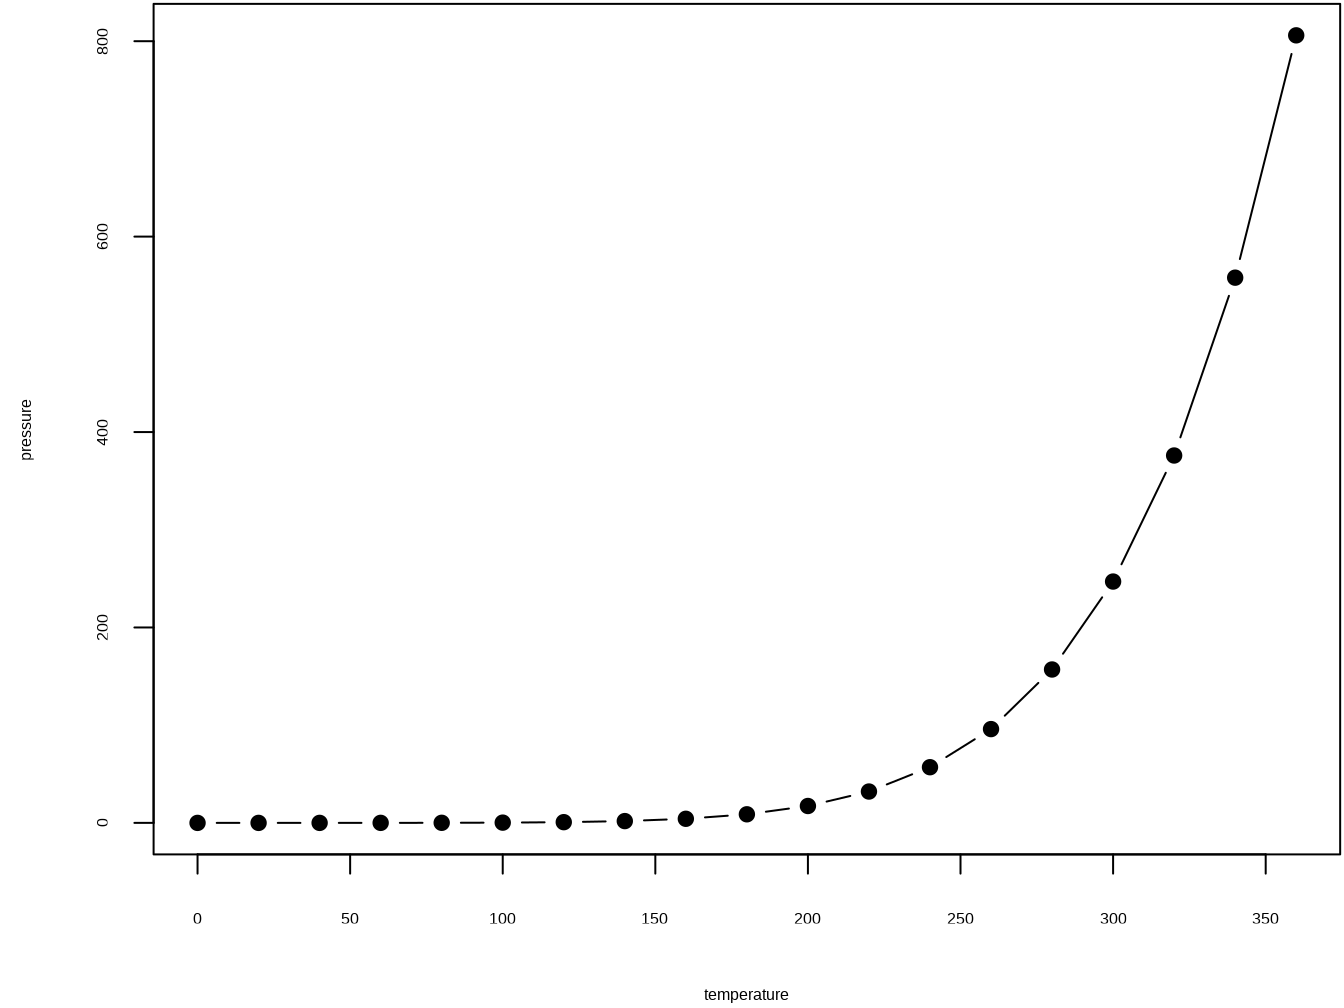
\includegraphics[width=0.8\linewidth]{02-cross-refs_files/figure-latex/nice-fig-1} 

}

\caption{Here is a nice figure!}\label{fig:nice-fig}
\end{figure}

Don't miss Table \ref{tab:nice-tab}.

\begin{Shaded}
\begin{Highlighting}[]
\NormalTok{knitr}\SpecialCharTok{::}\FunctionTok{kable}\NormalTok{(}
  \FunctionTok{head}\NormalTok{(pressure, }\DecValTok{10}\NormalTok{), }\AttributeTok{caption =} \StringTok{\textquotesingle{}Here is a nice table!\textquotesingle{}}\NormalTok{,}
  \AttributeTok{booktabs =} \ConstantTok{TRUE}
\NormalTok{)}
\end{Highlighting}
\end{Shaded}

\begin{table}

\caption{\label{tab:nice-tab}Here is a nice table!}
\centering
\begin{tabular}[t]{rr}
\toprule
temperature & pressure\\
\midrule
0 & 0.0002\\
20 & 0.0012\\
40 & 0.0060\\
60 & 0.0300\\
80 & 0.0900\\
\addlinespace
100 & 0.2700\\
120 & 0.7500\\
140 & 1.8500\\
160 & 4.2000\\
180 & 8.8000\\
\bottomrule
\end{tabular}
\end{table}

\hypertarget{parts}{%
\chapter{Parts}\label{parts}}

You can add parts to organize one or more book chapters together. Parts can be inserted at the top of an .Rmd file, before the first-level chapter heading in that same file.

Add a numbered part: \texttt{\#\ (PART)\ Act\ one\ \{-\}} (followed by \texttt{\#\ A\ chapter})

Add an unnumbered part: \texttt{\#\ (PART\textbackslash{}*)\ Act\ one\ \{-\}} (followed by \texttt{\#\ A\ chapter})

Add an appendix as a special kind of un-numbered part: \texttt{\#\ (APPENDIX)\ Other\ stuff\ \{-\}} (followed by \texttt{\#\ A\ chapter}). Chapters in an appendix are prepended with letters instead of numbers.

\hypertarget{footnotes-and-citations}{%
\chapter{Footnotes and citations}\label{footnotes-and-citations}}

\hypertarget{footnotes}{%
\section{Footnotes}\label{footnotes}}

Footnotes are put inside the square brackets after a caret \texttt{\^{}{[}{]}}. Like this one \footnote{This is a footnote.}.

\hypertarget{citations}{%
\section{Citations}\label{citations}}

Reference items in your bibliography file(s) using \texttt{@key}.

For example, we are using the \textbf{bookdown} package \citep{R-bookdown} (check out the last code chunk in index.Rmd to see how this citation key was added) in this sample book, which was built on top of R Markdown and \textbf{knitr} \citep{xie2015} (this citation was added manually in an external file book.bib).
Note that the \texttt{.bib} files need to be listed in the index.Rmd with the YAML \texttt{bibliography} key.

The \texttt{bs4\_book} theme makes footnotes appear inline when you click on them. In this example book, we added \texttt{csl:\ chicago-fullnote-bibliography.csl} to the \texttt{index.Rmd} YAML, and include the \texttt{.csl} file. To download a new style, we recommend: \url{https://www.zotero.org/styles/}

The RStudio Visual Markdown Editor can also make it easier to insert citations: \url{https://rstudio.github.io/visual-markdown-editing/\#/citations}

\hypertarget{blocks}{%
\chapter{Blocks}\label{blocks}}

\hypertarget{equations}{%
\section{Equations}\label{equations}}

Here is an equation.

\begin{equation} 
  f\left(k\right) = \binom{n}{k} p^k\left(1-p\right)^{n-k}
  \label{eq:binom}
\end{equation}

You may refer to using \texttt{\textbackslash{}@ref(eq:binom)}, like see Equation \eqref{eq:binom}.

\hypertarget{theorems-and-proofs}{%
\section{Theorems and proofs}\label{theorems-and-proofs}}

Labeled theorems can be referenced in text using \texttt{\textbackslash{}@ref(thm:tri)}, for example, check out this smart theorem \ref{thm:tri}.

\begin{theorem}
\protect\hypertarget{thm:tri}{}\label{thm:tri}For a right triangle, if \(c\) denotes the \emph{length} of the hypotenuse
and \(a\) and \(b\) denote the lengths of the \textbf{other} two sides, we have
\[a^2 + b^2 = c^2\]
\end{theorem}

Read more here \url{https://bookdown.org/yihui/bookdown/markdown-extensions-by-bookdown.html}.

\hypertarget{callout-blocks}{%
\section{Callout blocks}\label{callout-blocks}}

The \texttt{bs4\_book} theme also includes special callout blocks, like this \texttt{.rmdnote}.

You can use \textbf{markdown} inside a block.

\begin{Shaded}
\begin{Highlighting}[]
\FunctionTok{head}\NormalTok{(beaver1, }\AttributeTok{n =} \DecValTok{5}\NormalTok{)}
\CommentTok{\#\textgreater{}   day time  temp activ}
\CommentTok{\#\textgreater{} 1 346  840 36.33     0}
\CommentTok{\#\textgreater{} 2 346  850 36.34     0}
\CommentTok{\#\textgreater{} 3 346  900 36.35     0}
\CommentTok{\#\textgreater{} 4 346  910 36.42     0}
\CommentTok{\#\textgreater{} 5 346  920 36.55     0}
\end{Highlighting}
\end{Shaded}

It is up to the user to define the appearance of these blocks for LaTeX output.

You may also use: \texttt{.rmdcaution}, \texttt{.rmdimportant}, \texttt{.rmdtip}, or \texttt{.rmdwarning} as the block name.

The R Markdown Cookbook provides more help on how to use custom blocks to design your own callouts: \url{https://bookdown.org/yihui/rmarkdown-cookbook/custom-blocks.html}

\hypertarget{sharing-your-book}{%
\chapter{Sharing your book}\label{sharing-your-book}}

\hypertarget{publishing}{%
\section{Publishing}\label{publishing}}

HTML books can be published online, see: \url{https://bookdown.org/yihui/bookdown/publishing.html}

\hypertarget{pages}{%
\section{404 pages}\label{pages}}

By default, users will be directed to a 404 page if they try to access a webpage that cannot be found. If you'd like to customize your 404 page instead of using the default, you may add either a \texttt{\_404.Rmd} or \texttt{\_404.md} file to your project root and use code and/or Markdown syntax.

\hypertarget{metadata-for-sharing}{%
\section{Metadata for sharing}\label{metadata-for-sharing}}

Bookdown HTML books will provide HTML metadata for social sharing on platforms like Twitter, Facebook, and LinkedIn, using information you provide in the \texttt{index.Rmd} YAML. To setup, set the \texttt{url} for your book and the path to your \texttt{cover-image} file. Your book's \texttt{title} and \texttt{description} are also used.

This \texttt{bs4\_book} provides enhanced metadata for social sharing, so that each chapter shared will have a unique description, auto-generated based on the content.

Specify your book's source repository on GitHub as the \texttt{repo} in the \texttt{\_output.yml} file, which allows users to view each chapter's source file or suggest an edit. Read more about the features of this output format here:

\url{https://pkgs.rstudio.com/bookdown/reference/bs4_book.html}

Or use:

\begin{Shaded}
\begin{Highlighting}[]
\NormalTok{?bookdown}\SpecialCharTok{::}\NormalTok{bs4\_book}
\end{Highlighting}
\end{Shaded}

\hypertarget{maps}{%
\chapter{作図}\label{maps}}

\begin{Shaded}
\begin{Highlighting}[]
\FunctionTok{library}\NormalTok{(tidyverse) }\CommentTok{\# Essential package}
\CommentTok{\#\textgreater{} {-}{-} Attaching packages {-}{-}{-}{-}{-}{-}{-}{-}{-}{-}{-}{-}{-}{-}{-}{-}{-}{-}{-} tidyverse 1.3.1 {-}{-}}
\CommentTok{\#\textgreater{} v ggplot2 3.3.5     v purrr   0.3.4}
\CommentTok{\#\textgreater{} v tibble  3.1.6     v dplyr   1.0.8}
\CommentTok{\#\textgreater{} v tidyr   1.2.0     v stringr 1.4.0}
\CommentTok{\#\textgreater{} v readr   2.1.2     v forcats 0.5.1}
\CommentTok{\#\textgreater{} {-}{-} Conflicts {-}{-}{-}{-}{-}{-}{-}{-}{-}{-}{-}{-}{-}{-}{-}{-}{-}{-}{-}{-}{-}{-} tidyverse\_conflicts() {-}{-}}
\CommentTok{\#\textgreater{} x dplyr::filter() masks stats::filter()}
\CommentTok{\#\textgreater{} x dplyr::lag()    masks stats::lag()}
\FunctionTok{library}\NormalTok{(ggpubr)     }\CommentTok{\# Publication{-}oriented figures}
\FunctionTok{library}\NormalTok{(kableExtra) }\CommentTok{\# Tables}
\CommentTok{\#\textgreater{} }
\CommentTok{\#\textgreater{} Attaching package: \textquotesingle{}kableExtra\textquotesingle{}}
\CommentTok{\#\textgreater{} The following object is masked from \textquotesingle{}package:dplyr\textquotesingle{}:}
\CommentTok{\#\textgreater{} }
\CommentTok{\#\textgreater{}     group\_rows}
\FunctionTok{library}\NormalTok{(magick)     }\CommentTok{\# Imagemagick R API}
\CommentTok{\#\textgreater{} Linking to ImageMagick 6.9.11.60}
\CommentTok{\#\textgreater{} Enabled features: fontconfig, freetype, fftw, heic, lcms, pango, webp, x11}
\CommentTok{\#\textgreater{} Disabled features: cairo, ghostscript, raw, rsvg}
\CommentTok{\#\textgreater{} Using 32 threads}
\FunctionTok{library}\NormalTok{(patchwork)  }\CommentTok{\# Simplified figure tiling}
\FunctionTok{library}\NormalTok{(ggspatial)  }\CommentTok{\# Essential for map{-}making with ggplot}
\FunctionTok{library}\NormalTok{(sf)         }\CommentTok{\# Essential for map data manipulation}
\CommentTok{\#\textgreater{} Linking to GEOS 3.9.0, GDAL 3.2.2, PROJ 7.2.1; sf\_use\_s2() is TRUE}
\FunctionTok{library}\NormalTok{(showtext)   }\CommentTok{\# I want to use google fonts in the figures}
\CommentTok{\#\textgreater{} Loading required package: sysfonts}
\CommentTok{\#\textgreater{} Loading required package: showtextdb}
\end{Highlighting}
\end{Shaded}

Noto Sans のフォントが好きなので、ここで \href{https://fonts.google.com/}{Google Fonts} からアクセスします。

\begin{Shaded}
\begin{Highlighting}[]
\FunctionTok{font\_add\_google}\NormalTok{(}\StringTok{"Noto Sans"}\NormalTok{,}\StringTok{"notosans"}\NormalTok{)}
\end{Highlighting}
\end{Shaded}

\texttt{ggplot} のデフォルトテーマも設定し、フォント埋め込みも可能にします。
ここでデフォルトを設定すると、毎回 \texttt{theme\_pubr()} を \texttt{ggplot}のチェインにたさなくていい。

\begin{Shaded}
\begin{Highlighting}[]
\FunctionTok{theme\_pubr}\NormalTok{(}\AttributeTok{base\_size =} \DecValTok{10}\NormalTok{, }\AttributeTok{base\_family =} \StringTok{"notosans"}\NormalTok{) }\SpecialCharTok{|}\ErrorTok{\textgreater{}} \FunctionTok{theme\_set}\NormalTok{()}
\FunctionTok{showtext\_auto}\NormalTok{() }\CommentTok{\# Automatically embed the Noto Sans fonts into the ggplots.}
\end{Highlighting}
\end{Shaded}

\hypertarget{ux30b7ux30a7ux30fcux30d7ux30d5ux30a1ux30a4ux30ebux306eux8aadux307fux8fbcux307f}{%
\section{シェープファイルの読み込み}\label{ux30b7ux30a7ux30fcux30d7ux30d5ux30a1ux30a4ux30ebux306eux8aadux307fux8fbcux307f}}

シェープファイル (shapefile) は地図データのことです。
基本的の拡張子は \texttt{shp}, \texttt{shx}, \texttt{dbf} ですが、その他に \texttt{prj} と \texttt{xml} もあります。

研究室用にダウンロードした \href{https://nlftp.mlit.go.jp/ksj/index.html}{国土交通省・国土数値情報ダウンロードサービス} のシェープファイルは \texttt{\textasciitilde{}/Lab\_Data/Japan\_map\_data/Japan} に入っています。

\begin{Shaded}
\begin{Highlighting}[]
\NormalTok{mlit }\OtherTok{=} \FunctionTok{read\_sf}\NormalTok{(}\StringTok{"\textasciitilde{}/Lab\_Data/Japan\_map\_data/Japan/N03{-}20210101\_GML/"}\NormalTok{)}
\end{Highlighting}
\end{Shaded}

\texttt{mlit} に読み込んだシェープファイルは\href{https://nlftp.mlit.go.jp/ksj/gml/datalist/KsjTmplt-N03-v3_0.html}{ここへ}。

シェープファイルの 座標参照系 (CRS: Coordinate Reference System) を確認しましょう。

\begin{Shaded}
\begin{Highlighting}[]
\FunctionTok{st\_crs}\NormalTok{(mlit)}
\CommentTok{\#\textgreater{} Coordinate Reference System:}
\CommentTok{\#\textgreater{}   User input: JGD2011 }
\CommentTok{\#\textgreater{}   wkt:}
\CommentTok{\#\textgreater{} GEOGCRS["JGD2011",}
\CommentTok{\#\textgreater{}     DATUM["Japanese Geodetic Datum 2011",}
\CommentTok{\#\textgreater{}         ELLIPSOID["GRS 1980",6378137,298.257222101,}
\CommentTok{\#\textgreater{}             LENGTHUNIT["metre",1]]],}
\CommentTok{\#\textgreater{}     PRIMEM["Greenwich",0,}
\CommentTok{\#\textgreater{}         ANGLEUNIT["degree",0.0174532925199433]],}
\CommentTok{\#\textgreater{}     CS[ellipsoidal,2],}
\CommentTok{\#\textgreater{}         AXIS["geodetic latitude (Lat)",north,}
\CommentTok{\#\textgreater{}             ORDER[1],}
\CommentTok{\#\textgreater{}             ANGLEUNIT["degree",0.0174532925199433]],}
\CommentTok{\#\textgreater{}         AXIS["geodetic longitude (Lon)",east,}
\CommentTok{\#\textgreater{}             ORDER[2],}
\CommentTok{\#\textgreater{}             ANGLEUNIT["degree",0.0174532925199433]],}
\CommentTok{\#\textgreater{}     USAGE[}
\CommentTok{\#\textgreater{}         SCOPE["Horizontal component of 3D system."],}
\CommentTok{\#\textgreater{}         AREA["Japan {-} onshore and offshore."],}
\CommentTok{\#\textgreater{}         BBOX[17.09,122.38,46.05,157.65]],}
\CommentTok{\#\textgreater{}     ID["EPSG",6668]]}
\end{Highlighting}
\end{Shaded}

CRSには \textbf{地理座標系} と \textbf{投影座標系} の2種類があります。
座標系にはEPSGコードもつけられています。

\begin{Shaded}
\begin{Highlighting}[]
\CommentTok{\# HTML 用テーブル}
\FunctionTok{tibble}\NormalTok{(}\StringTok{\textasciigrave{}}\AttributeTok{EPSG Code}\StringTok{\textasciigrave{}} \OtherTok{=} \FunctionTok{c}\NormalTok{(}\DecValTok{4326}\NormalTok{,}\DecValTok{6668}\NormalTok{,}\DecValTok{6677}\NormalTok{),}
       \StringTok{\textasciigrave{}}\AttributeTok{CRS}\StringTok{\textasciigrave{}} \OtherTok{=} \FunctionTok{c}\NormalTok{(}\StringTok{"WGS84"}\NormalTok{, }\StringTok{"JGD2011"}\NormalTok{, }\StringTok{"JGD2011 / Japan Plane Rectangular CS IX"}\NormalTok{),}
       \StringTok{\textasciigrave{}}\AttributeTok{Units}\StringTok{\textasciigrave{}} \OtherTok{=} \FunctionTok{c}\NormalTok{(}\StringTok{"degrees"}\NormalTok{, }\StringTok{"degrees"}\NormalTok{, }\StringTok{"meters"}\NormalTok{)) }\SpecialCharTok{|}\ErrorTok{\textgreater{}} 
  \FunctionTok{kbl}\NormalTok{() }\SpecialCharTok{|}\ErrorTok{\textgreater{}} 
  \FunctionTok{kable\_styling}\NormalTok{(}\AttributeTok{bootstrap\_options =} \FunctionTok{c}\NormalTok{(}\StringTok{"hover"}\NormalTok{))}
\end{Highlighting}
\end{Shaded}

\begin{table}
\centering
\begin{tabular}[t]{r|l|l}
\hline
EPSG Code & CRS & Units\\
\hline
4326 & WGS84 & degrees\\
\hline
6668 & JGD2011 & degrees\\
\hline
6677 & JGD2011 / Japan Plane Rectangular CS IX & meters\\
\hline
\end{tabular}
\end{table}

このデータは政策区域のデータなので、とても重いです。
まずは、都道府県ごとにまとめた \texttt{RDS} ファイルを作って保存します。
都道府県ごとに \texttt{st\_union()} を使って \texttt{polgyon} データを結合します。
結合したデータを unnest して、simple feature に戻してかた保存します。
121158 features もあるので、数時間もかります。

沿岸のデータだけなら軽いですので、\texttt{C23} シリーズのファイルを読み込みます。

\begin{Shaded}
\begin{Highlighting}[]
\NormalTok{mlit }\OtherTok{=} \FunctionTok{tibble}\NormalTok{(}\AttributeTok{folder =} \FunctionTok{dir}\NormalTok{(}\StringTok{"\textasciitilde{}/Lab\_Data/Japan\_map\_data/Coastline/"}\NormalTok{, }\AttributeTok{full =} \ConstantTok{TRUE}\NormalTok{)) }\SpecialCharTok{|}\ErrorTok{\textgreater{}} 
  \FunctionTok{mutate}\NormalTok{(}\AttributeTok{data =} \FunctionTok{map}\NormalTok{(folder, read\_sf)) }\SpecialCharTok{|}\ErrorTok{\textgreater{}} \FunctionTok{select}\NormalTok{(data) }\SpecialCharTok{|}\ErrorTok{\textgreater{}} 
  \FunctionTok{unnest}\NormalTok{(data) }\SpecialCharTok{|}\ErrorTok{\textgreater{}} 
  \FunctionTok{st\_as\_sf}\NormalTok{(}\AttributeTok{crs =} \FunctionTok{st\_crs}\NormalTok{(}\DecValTok{6668}\NormalTok{))}
\end{Highlighting}
\end{Shaded}

では、ここで地図の確認をします。

\begin{Shaded}
\begin{Highlighting}[]
\NormalTok{mlit }\SpecialCharTok{|}\ErrorTok{\textgreater{}} \FunctionTok{ggplot}\NormalTok{() }\SpecialCharTok{+} \FunctionTok{geom\_sf}\NormalTok{()}
\end{Highlighting}
\end{Shaded}

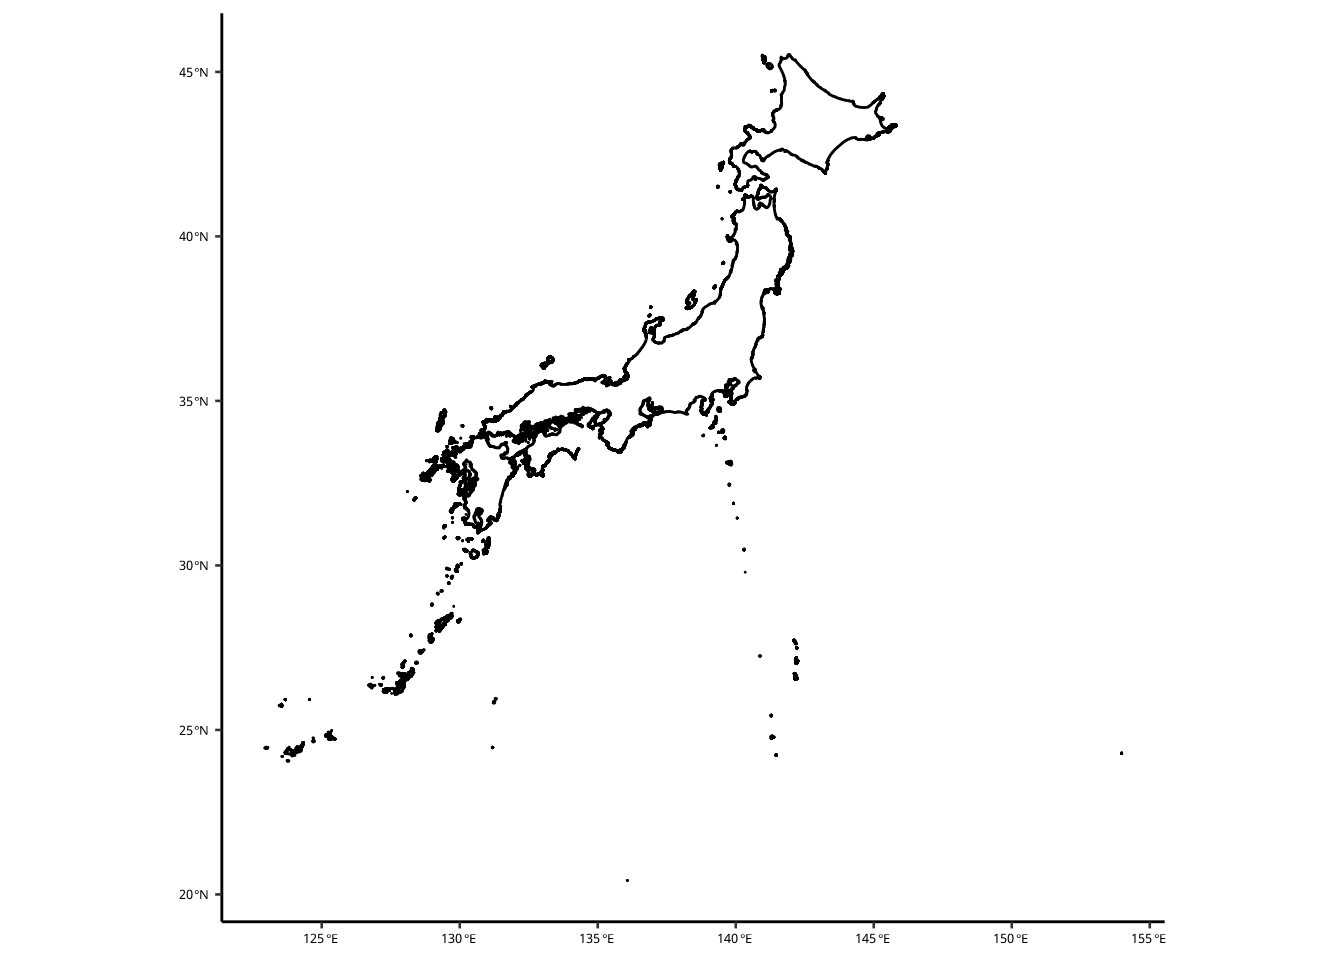
\includegraphics{50-maps_files/figure-latex/unnamed-chunk-7-1.pdf}

\texttt{mlit} のデータは細かい政策区域まで分けられているので、全国スケールの図には向いていません。
\texttt{st\_union()} をつかって、都道府県ごとに polygon を結合したファイルは、\texttt{\textasciitilde{}/Lab\_Data/Japan\_map\_data/Japan/todofuken.rds} に保存しています。
次のコードで、都道府県ごとにまとめましたが、並列処理でも5時間以上もかかったので、\texttt{RDS} ファイルを使いましょう。

\begin{Shaded}
\begin{Highlighting}[]
\CommentTok{\# Takes 5.5 hours to complete with 30 cores!}
\FunctionTok{library}\NormalTok{(furrr)}
\FunctionTok{plan}\NormalTok{(multisession, }\AttributeTok{workers =} \DecValTok{30}\NormalTok{)}
\CommentTok{\# Group by prefecture}
\NormalTok{mlit1 }\OtherTok{=}\NormalTok{ mlit }\SpecialCharTok{|}\ErrorTok{\textgreater{}} \FunctionTok{group\_nest}\NormalTok{(N03\_001) }\SpecialCharTok{|}\ErrorTok{\textgreater{}} 
  \FunctionTok{mutate}\NormalTok{(}\AttributeTok{data =} \FunctionTok{future\_map}\NormalTok{(data, st\_union)) }\SpecialCharTok{|}\ErrorTok{\textgreater{}} 
  \FunctionTok{unnest}\NormalTok{(data) }\SpecialCharTok{|}\ErrorTok{\textgreater{}} \FunctionTok{st\_as\_sf}\NormalTok{() }
\NormalTok{mlit1 }\SpecialCharTok{|}\ErrorTok{\textgreater{}} \FunctionTok{write\_rds}\NormalTok{(}\StringTok{"\textasciitilde{}/Lab\_Data/Japan\_map\_data/Japan/todofuken.rds"}\NormalTok{)}
\end{Highlighting}
\end{Shaded}

\begin{Shaded}
\begin{Highlighting}[]
\NormalTok{mlit1 }\OtherTok{=} \FunctionTok{read\_rds}\NormalTok{(}\StringTok{"\textasciitilde{}/Lab\_Data/Japan\_map\_data/Japan/todofuken.rds"}\NormalTok{)}
\end{Highlighting}
\end{Shaded}

\begin{Shaded}
\begin{Highlighting}[]
\NormalTok{mlit1 }\SpecialCharTok{|}\ErrorTok{\textgreater{}} \FunctionTok{ggplot}\NormalTok{() }\SpecialCharTok{+} \FunctionTok{geom\_sf}\NormalTok{()}
\end{Highlighting}
\end{Shaded}

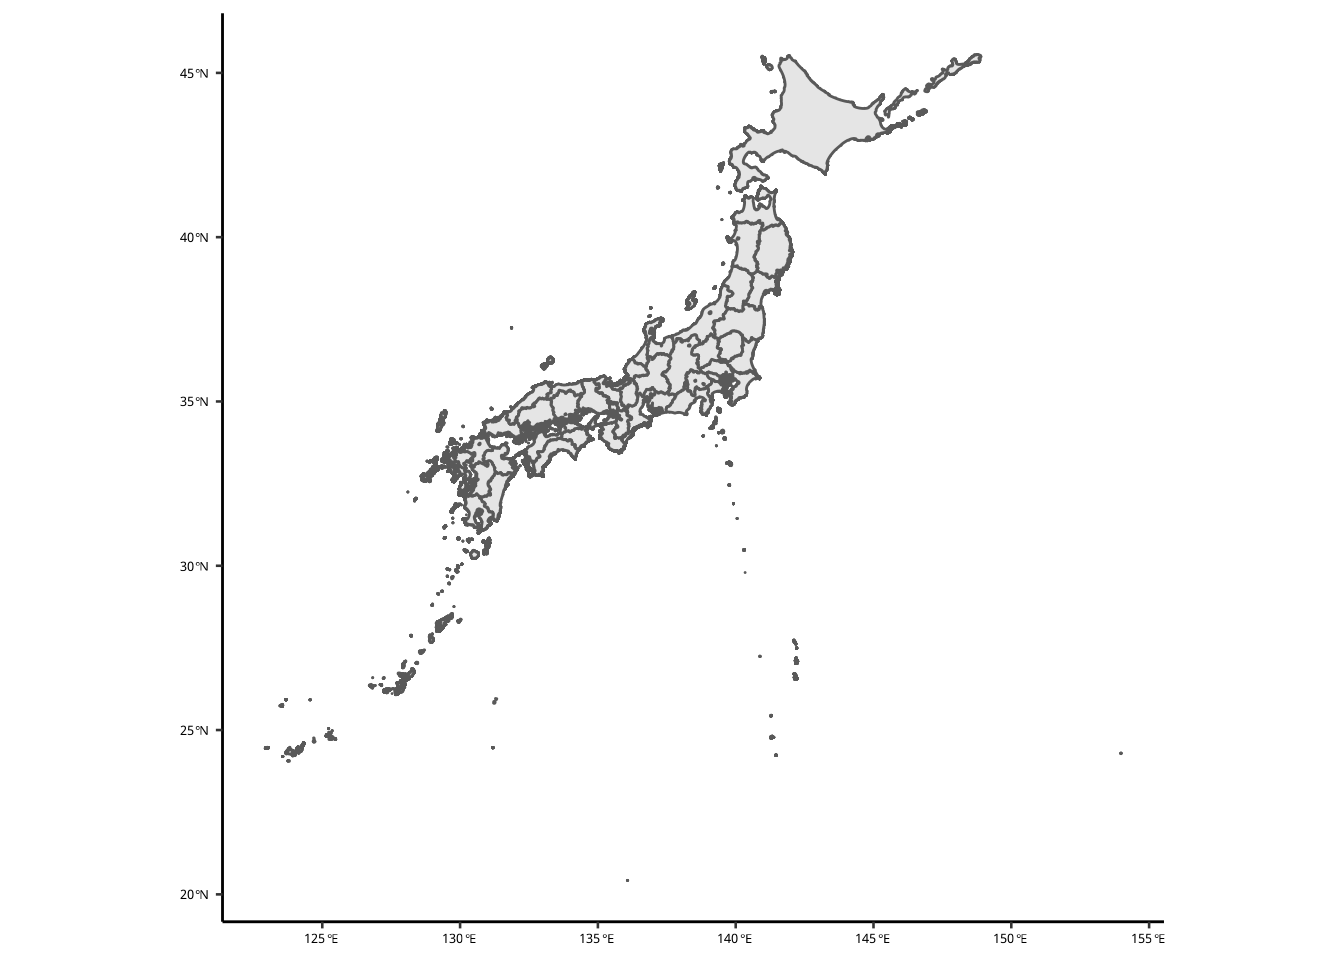
\includegraphics{50-maps_files/figure-latex/unnamed-chunk-10-1.pdf}

\hypertarget{ux8abfux67fbux5730ux70b9ux306eux30c7ux30fcux30bfux3092ux6e96ux5099ux3059ux308b}{%
\section{調査地点のデータを準備する}\label{ux8abfux67fbux5730ux70b9ux306eux30c7ux30fcux30bfux3092ux6e96ux5099ux3059ux308b}}

形上湾アマモ場調査のステーションの GPS \texttt{tibble} を準備する。

\begin{Shaded}
\begin{Highlighting}[]
\NormalTok{zostera }\OtherTok{=} \FunctionTok{read\_csv}\NormalTok{(}\StringTok{"\textasciitilde{}/Lab\_Data/matsumuro/Katagami\_Bay/longlat\_info.csv"}\NormalTok{)}
\CommentTok{\#\textgreater{} Rows: 105 Columns: 6}
\CommentTok{\#\textgreater{} {-}{-} Column specification {-}{-}{-}{-}{-}{-}{-}{-}{-}{-}{-}{-}{-}{-}{-}{-}{-}{-}{-}{-}{-}{-}{-}{-}{-}{-}{-}{-}{-}{-}{-}{-}{-}{-}{-}{-}}
\CommentTok{\#\textgreater{} Delimiter: ","}
\CommentTok{\#\textgreater{} chr  (1): eelgrass}
\CommentTok{\#\textgreater{} dbl  (4): Name, lat, long, coverage(\%)}
\CommentTok{\#\textgreater{} dttm (1): datetime}
\CommentTok{\#\textgreater{} }
\CommentTok{\#\textgreater{} i Use \textasciigrave{}spec()\textasciigrave{} to retrieve the full column specification for this data.}
\CommentTok{\#\textgreater{} i Specify the column types or set \textasciigrave{}show\_col\_types = FALSE\textasciigrave{} to quiet this message.}
\NormalTok{zostera }\SpecialCharTok{|}\ErrorTok{\textgreater{}} \FunctionTok{print}\NormalTok{(}\AttributeTok{n =} \DecValTok{3}\NormalTok{)}
\CommentTok{\#\textgreater{} \# A tibble: 105 x 6}
\CommentTok{\#\textgreater{}    Name   lat  long datetime            eelgrass}
\CommentTok{\#\textgreater{}   \textless{}dbl\textgreater{} \textless{}dbl\textgreater{} \textless{}dbl\textgreater{} \textless{}dttm\textgreater{}              \textless{}chr\textgreater{}   }
\CommentTok{\#\textgreater{} 1     1  33.0  130. 2021{-}05{-}25 09:14:48 absent  }
\CommentTok{\#\textgreater{} 2     2  33.0  130. 2021{-}05{-}25 09:30:32 absent  }
\CommentTok{\#\textgreater{} 3     3  33.0  130. 2021{-}05{-}25 09:37:16 present }
\CommentTok{\#\textgreater{} \# ... with 102 more rows, and 1 more variable:}
\CommentTok{\#\textgreater{} \#   \textasciigrave{}coverage(\%)\textasciigrave{} \textless{}dbl\textgreater{}}
\end{Highlighting}
\end{Shaded}

\texttt{zostera} に緯度経度を設定する。
CRS は \texttt{mlit} と同じにします。

\begin{Shaded}
\begin{Highlighting}[]
\NormalTok{zostera }\OtherTok{=}\NormalTok{ zostera }\SpecialCharTok{|}\ErrorTok{\textgreater{}} \FunctionTok{st\_as\_sf}\NormalTok{(}\AttributeTok{coords =} \FunctionTok{c}\NormalTok{(}\StringTok{"long"}\NormalTok{, }\StringTok{"lat"}\NormalTok{), }\AttributeTok{crs =} \FunctionTok{st\_crs}\NormalTok{(mlit))}
\NormalTok{zostera }\SpecialCharTok{|}\ErrorTok{\textgreater{}} \FunctionTok{print}\NormalTok{(}\AttributeTok{n =} \DecValTok{3}\NormalTok{)}
\CommentTok{\#\textgreater{} Simple feature collection with 105 features and 4 fields}
\CommentTok{\#\textgreater{} Geometry type: POINT}
\CommentTok{\#\textgreater{} Dimension:     XY}
\CommentTok{\#\textgreater{} Bounding box:  xmin: 129.7845 ymin: 32.90032 xmax: 129.806 ymax: 32.95375}
\CommentTok{\#\textgreater{} Geodetic CRS:  JGD2011}
\CommentTok{\#\textgreater{} \# A tibble: 105 x 5}
\CommentTok{\#\textgreater{}    Name datetime            eelgrass \textasciigrave{}coverage(\%)\textasciigrave{}}
\CommentTok{\#\textgreater{} * \textless{}dbl\textgreater{} \textless{}dttm\textgreater{}              \textless{}chr\textgreater{}            \textless{}dbl\textgreater{}}
\CommentTok{\#\textgreater{} 1     1 2021{-}05{-}25 09:14:48 absent               0}
\CommentTok{\#\textgreater{} 2     2 2021{-}05{-}25 09:30:32 absent               0}
\CommentTok{\#\textgreater{} 3     3 2021{-}05{-}25 09:37:16 present              5}
\CommentTok{\#\textgreater{} \# ... with 102 more rows, and 1 more variable:}
\CommentTok{\#\textgreater{} \#   geometry \textless{}POINT [°]\textgreater{}}
\end{Highlighting}
\end{Shaded}

\hypertarget{ux4e5dux5ddeux30c7ux30fcux30bfux306eux62bdux51fa}{%
\section{九州データの抽出}\label{ux4e5dux5ddeux30c7ux30fcux30bfux306eux62bdux51fa}}

九州のデータと長崎のデータを抽出します。
\textbf{重要:長崎の名前が誤っています。\texttt{Nagasaki} のはずが、\texttt{Naoasaki} として記録されています。}

\begin{Shaded}
\begin{Highlighting}[]
\NormalTok{toget }\OtherTok{=} \StringTok{"長崎|福岡|大分|佐賀|熊本|鹿児島|宮崎"}
\NormalTok{kyushu }\OtherTok{=}\NormalTok{ mlit1 }\SpecialCharTok{|}\ErrorTok{\textgreater{}} \FunctionTok{filter}\NormalTok{(}\FunctionTok{str\_detect}\NormalTok{(N03\_001, toget))}
\end{Highlighting}
\end{Shaded}

海岸線のデータ (\texttt{mlit}) から長崎の情報を抽出したいが、このデータの位置情報はコードで記述されています。

\begin{Shaded}
\begin{Highlighting}[]
\NormalTok{admincode }\OtherTok{=}\NormalTok{ readxl}\SpecialCharTok{::}\FunctionTok{read\_xlsx}\NormalTok{(}\StringTok{"\textasciitilde{}/Lab\_Data/Japan\_map\_data/AdminiBoundary\_CD.xlsx"}\NormalTok{, }\AttributeTok{skip =} \DecValTok{2}\NormalTok{)}
\NormalTok{admincode }\OtherTok{=}\NormalTok{ admincode }\SpecialCharTok{|}\ErrorTok{\textgreater{}} \FunctionTok{select}\NormalTok{(}\AttributeTok{code =} \FunctionTok{matches}\NormalTok{(}\StringTok{"行政"}\NormalTok{), }\AttributeTok{N03\_001 =} \FunctionTok{matches}\NormalTok{(}\StringTok{"都道府県*.*漢字"}\NormalTok{))}
\NormalTok{codes }\OtherTok{=}\NormalTok{ admincode }\SpecialCharTok{|}\ErrorTok{\textgreater{}} \FunctionTok{filter}\NormalTok{(}\FunctionTok{str\_detect}\NormalTok{(N03\_001, }\StringTok{"長崎"}\NormalTok{)) }\SpecialCharTok{|}\ErrorTok{\textgreater{}} \FunctionTok{pull}\NormalTok{(code)}
\end{Highlighting}
\end{Shaded}

\begin{Shaded}
\begin{Highlighting}[]
\NormalTok{nagasaki }\OtherTok{=}\NormalTok{ mlit }\SpecialCharTok{|}\ErrorTok{\textgreater{}} \FunctionTok{filter}\NormalTok{(}\FunctionTok{str\_detect}\NormalTok{(C23\_001, }\FunctionTok{str\_c}\NormalTok{(codes, }\AttributeTok{collapse =} \StringTok{"|"}\NormalTok{))) }
\end{Highlighting}
\end{Shaded}

長崎の海岸線は次のようになります。

\begin{Shaded}
\begin{Highlighting}[]
\FunctionTok{ggplot}\NormalTok{() }\SpecialCharTok{+} \FunctionTok{geom\_sf}\NormalTok{(}\AttributeTok{data =}\NormalTok{ nagasaki)}
\end{Highlighting}
\end{Shaded}

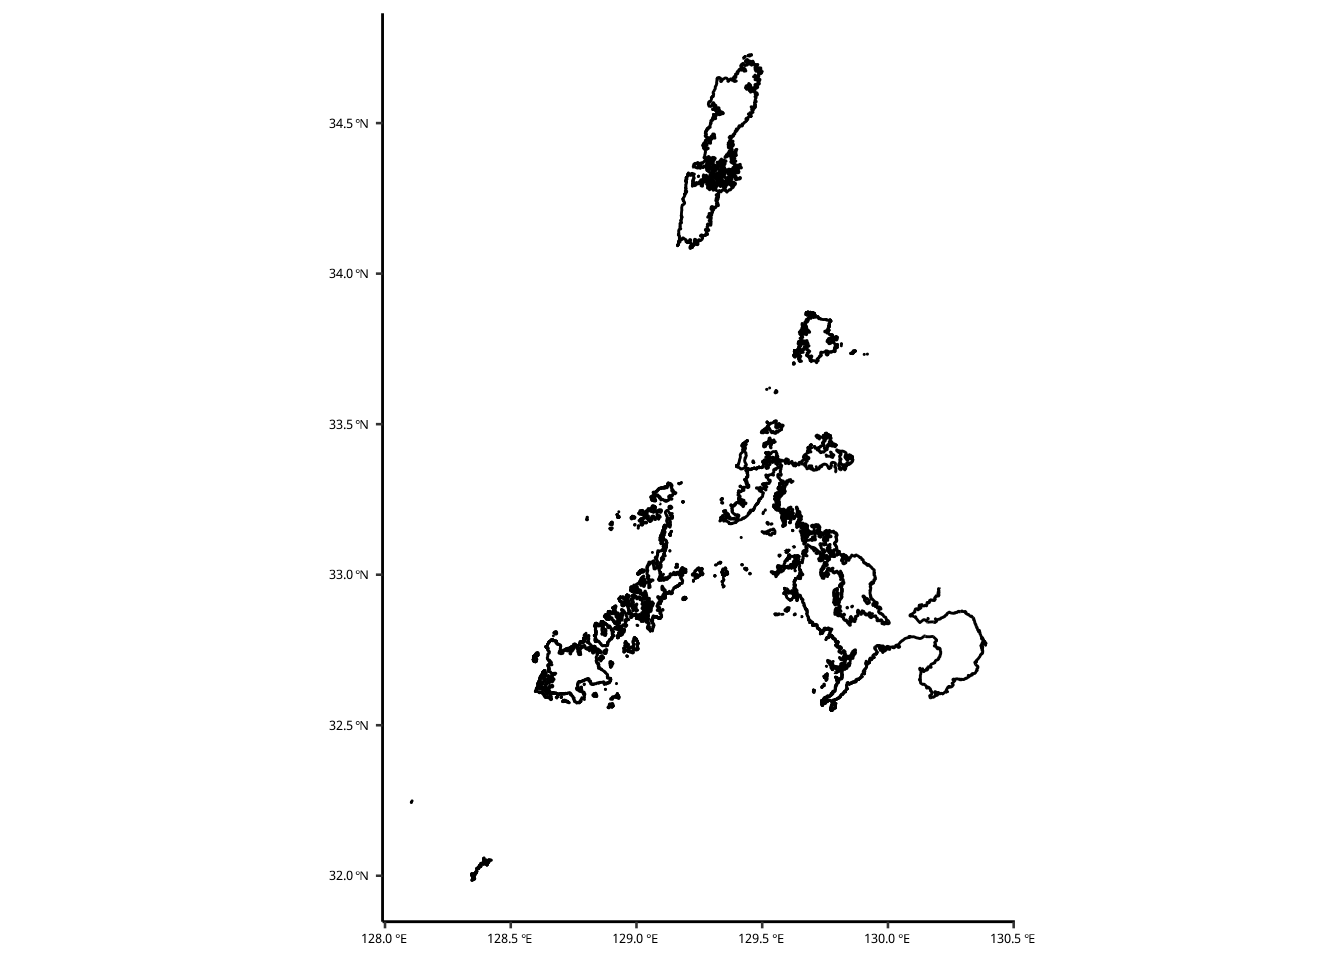
\includegraphics{50-maps_files/figure-latex/unnamed-chunk-16-1.pdf}

九州は \texttt{mlit1} から抽出したので、都道府県政策区域として作図されます。

\begin{Shaded}
\begin{Highlighting}[]
\FunctionTok{ggplot}\NormalTok{() }\SpecialCharTok{+} \FunctionTok{geom\_sf}\NormalTok{(}\AttributeTok{data =}\NormalTok{ kyushu)}
\end{Highlighting}
\end{Shaded}

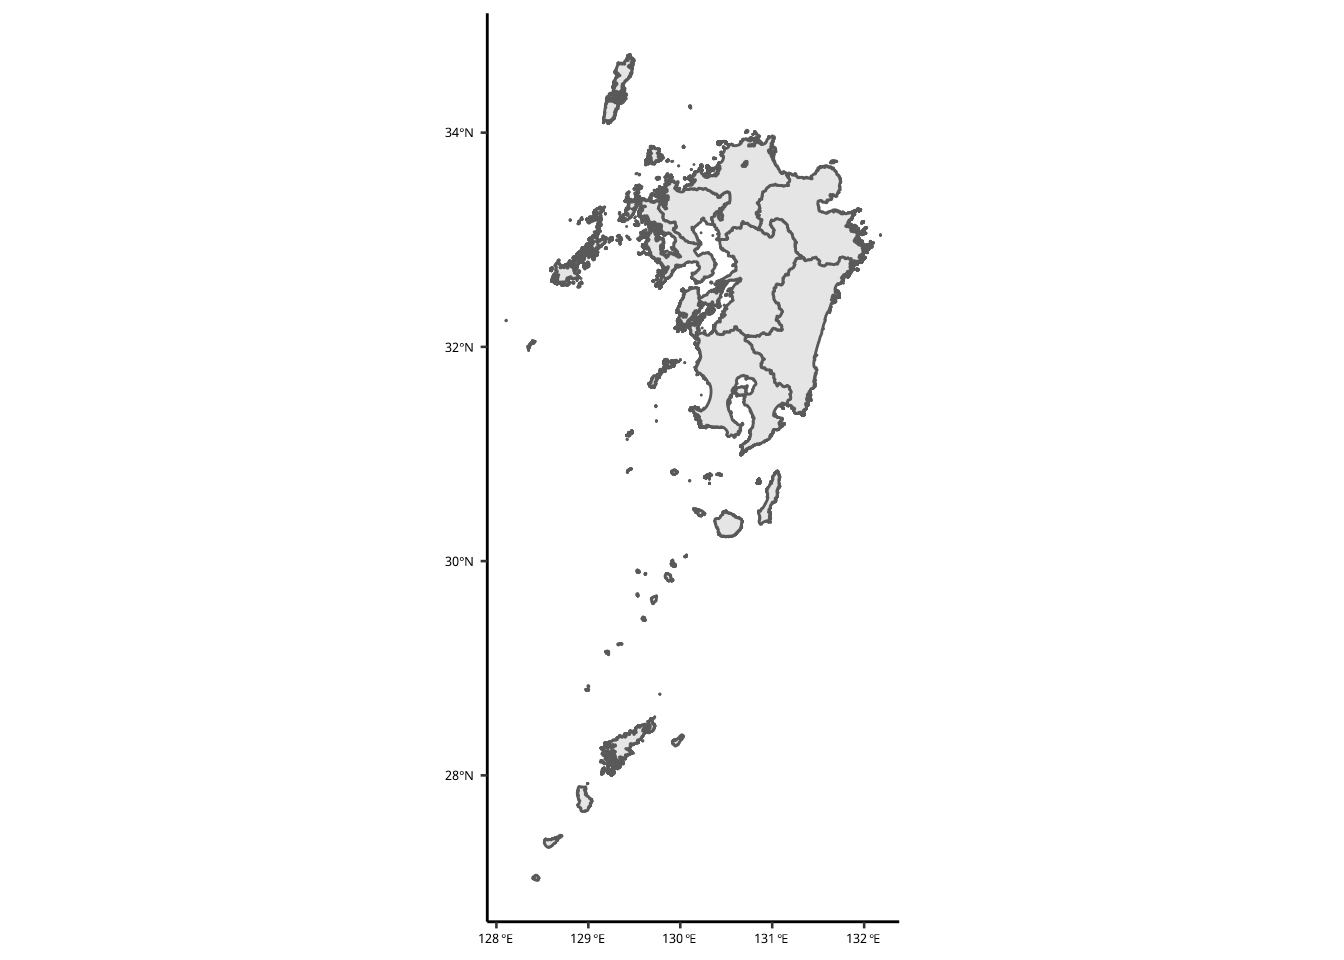
\includegraphics{50-maps_files/figure-latex/unnamed-chunk-17-1.pdf}

長崎をハイライトしましょう。

\begin{Shaded}
\begin{Highlighting}[]
\NormalTok{kyushu }\SpecialCharTok{|}\ErrorTok{\textgreater{}} 
  \FunctionTok{mutate}\NormalTok{(}\AttributeTok{fillme =} \FunctionTok{str\_detect}\NormalTok{(N03\_001, }\StringTok{"長崎"}\NormalTok{)) }\SpecialCharTok{|}\ErrorTok{\textgreater{}} 
  \FunctionTok{ggplot}\NormalTok{() }\SpecialCharTok{+} \FunctionTok{geom\_sf}\NormalTok{(}\FunctionTok{aes}\NormalTok{(}\AttributeTok{fill =}\NormalTok{ fillme), }\AttributeTok{color =} \ConstantTok{NA}\NormalTok{) }\SpecialCharTok{+}
  \FunctionTok{guides}\NormalTok{(}\AttributeTok{fill =} \StringTok{"none"}\NormalTok{) }\SpecialCharTok{+}
  \FunctionTok{scale\_fill\_viridis\_d}\NormalTok{() }\SpecialCharTok{+}
  \FunctionTok{theme}\NormalTok{(}\AttributeTok{panel.background =} \FunctionTok{element\_rect}\NormalTok{(}\AttributeTok{fill =} \StringTok{"lightblue"}\NormalTok{, }\AttributeTok{color =} \StringTok{"black"}\NormalTok{),}
        \AttributeTok{axis.line =} \FunctionTok{element\_blank}\NormalTok{())}
\end{Highlighting}
\end{Shaded}

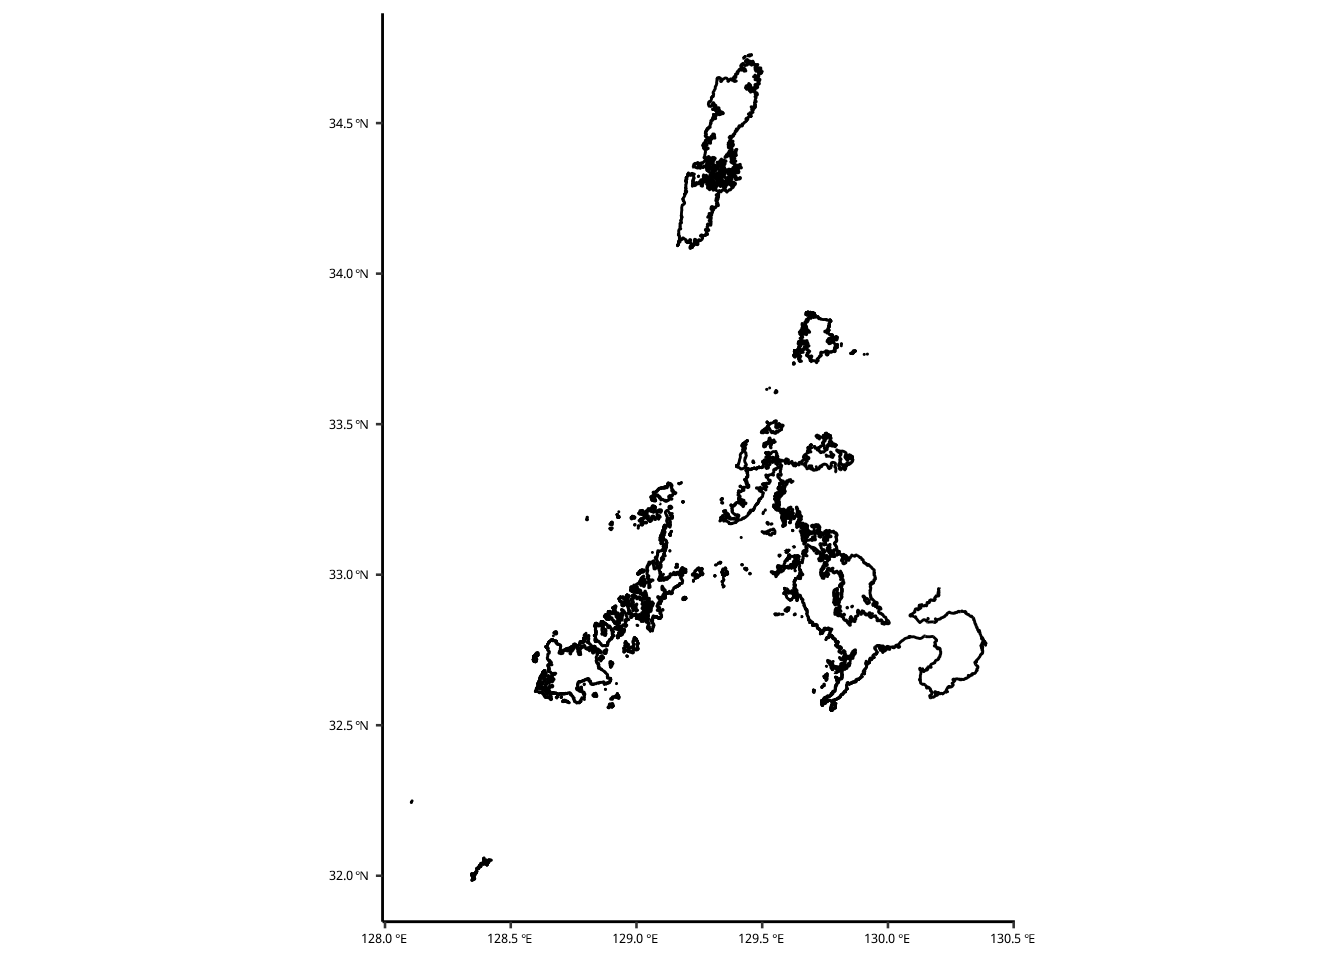
\includegraphics{50-maps_files/figure-latex/unnamed-chunk-18-1.pdf}

この図には、違和感を感じるので、山口、島根、愛媛、広島と高知も追加します。
そしれ、最初に作った \texttt{kyushu} の範囲を抽出しておきます。

\begin{Shaded}
\begin{Highlighting}[]
\NormalTok{kbbox }\OtherTok{=}\NormalTok{ kyushu }\SpecialCharTok{|}\ErrorTok{\textgreater{}} \FunctionTok{st\_bbox}\NormalTok{()}
\end{Highlighting}
\end{Shaded}

\begin{Shaded}
\begin{Highlighting}[]
\NormalTok{toget }\OtherTok{=} \StringTok{"長崎|福岡|大分|佐賀|熊本|鹿児島|宮崎|山口|島根|愛媛|高知|広島"}
\NormalTok{kyushu }\OtherTok{=}\NormalTok{ mlit1 }\SpecialCharTok{|}\ErrorTok{\textgreater{}} \FunctionTok{filter}\NormalTok{(}\FunctionTok{str\_detect}\NormalTok{(N03\_001, toget))}
\end{Highlighting}
\end{Shaded}

長崎、九州、その他の色分けをして、 \texttt{kyushu} をクロップします。
クロップ範囲は \texttt{kbbox} です。

\begin{Shaded}
\begin{Highlighting}[]
\NormalTok{kyushu }\OtherTok{=}\NormalTok{ kyushu }\SpecialCharTok{|}\ErrorTok{\textgreater{}}
  \FunctionTok{mutate}\NormalTok{(}\AttributeTok{fillme =} \FunctionTok{case\_when}\NormalTok{(}\FunctionTok{str\_detect}\NormalTok{(N03\_001, }\StringTok{"長崎"}\NormalTok{) }\SpecialCharTok{\textasciitilde{}} \StringTok{"Nagasaki"}\NormalTok{,}
                            \FunctionTok{str\_detect}\NormalTok{(N03\_001, }\StringTok{"福岡|大分|佐賀|熊本|鹿児島|宮崎"}\NormalTok{) }\SpecialCharTok{\textasciitilde{}} \StringTok{"Kyushu"}\NormalTok{,}
                            \ConstantTok{TRUE} \SpecialCharTok{\textasciitilde{}} \StringTok{"Honshu"}\NormalTok{)) }\SpecialCharTok{|}\ErrorTok{\textgreater{}} 
  \FunctionTok{st\_crop}\NormalTok{(kbbox)}
\CommentTok{\#\textgreater{} Warning: attribute variables are assumed to be spatially}
\CommentTok{\#\textgreater{} constant throughout all geometries}
\end{Highlighting}
\end{Shaded}

この地図は次のようになりました。

\begin{Shaded}
\begin{Highlighting}[]
\FunctionTok{ggplot}\NormalTok{(kyushu) }\SpecialCharTok{+} 
  \FunctionTok{geom\_sf}\NormalTok{(}\FunctionTok{aes}\NormalTok{(}\AttributeTok{fill =}\NormalTok{ fillme), }\AttributeTok{color =} \ConstantTok{NA}\NormalTok{) }\SpecialCharTok{+}
  \FunctionTok{guides}\NormalTok{(}\AttributeTok{fill =} \StringTok{"none"}\NormalTok{) }\SpecialCharTok{+}
  \FunctionTok{coord\_sf}\NormalTok{(}\AttributeTok{expand =} \ConstantTok{FALSE}\NormalTok{) }\SpecialCharTok{+}
  \FunctionTok{scale\_fill\_viridis\_d}\NormalTok{() }\SpecialCharTok{+}
  \FunctionTok{theme}\NormalTok{(}\AttributeTok{panel.background =} \FunctionTok{element\_rect}\NormalTok{(}\AttributeTok{fill =} \StringTok{"lightblue"}\NormalTok{, }\AttributeTok{color =} \StringTok{"black"}\NormalTok{),}
        \AttributeTok{axis.line =} \FunctionTok{element\_blank}\NormalTok{())}
\end{Highlighting}
\end{Shaded}

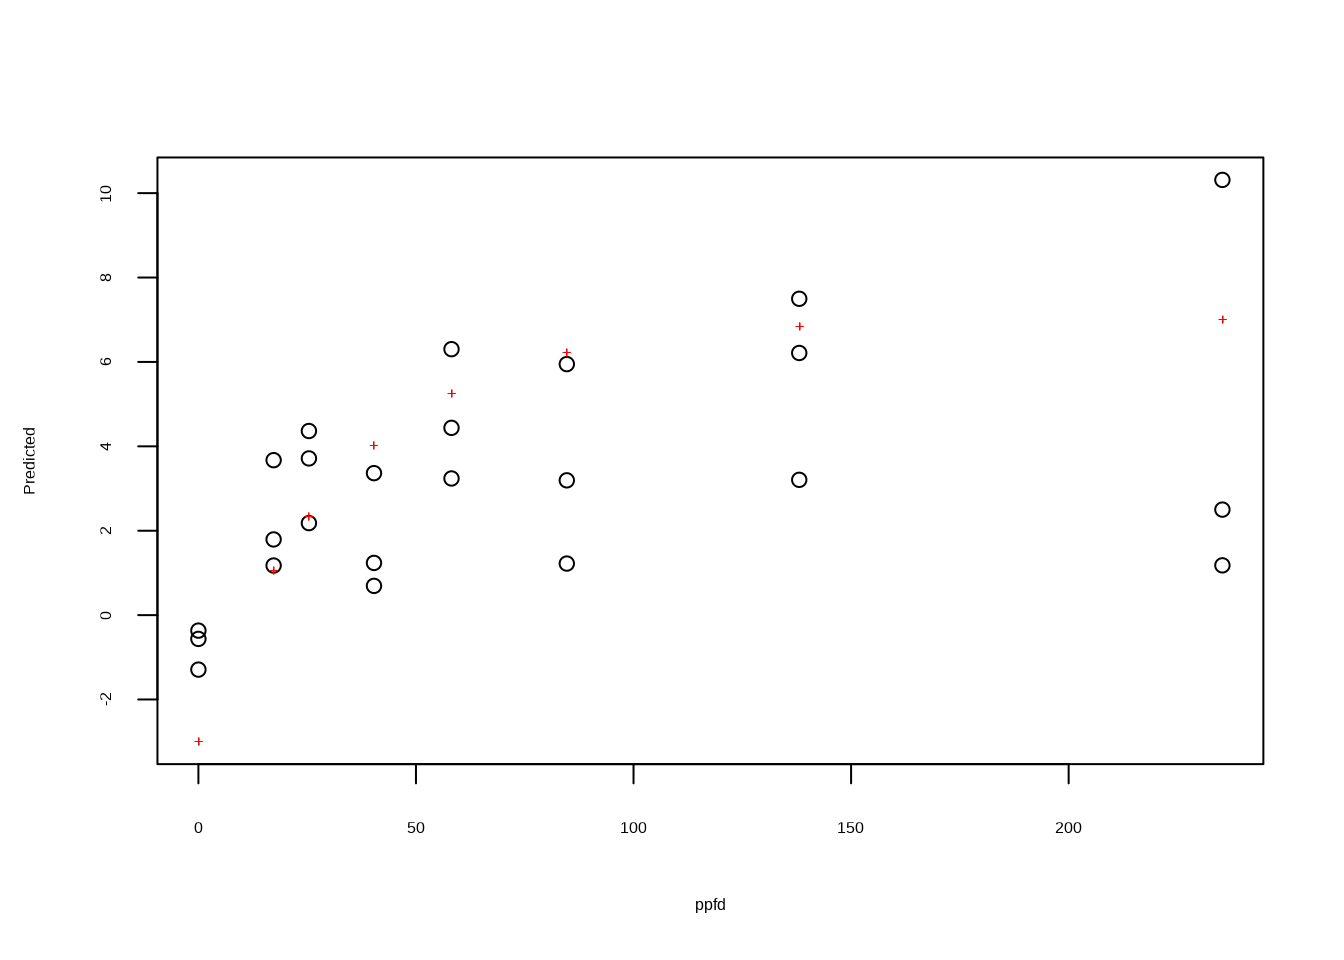
\includegraphics{50-maps_files/figure-latex/unnamed-chunk-22-1.pdf}

\hypertarget{ux8abfux67fbux5730ux70b9ux306eux56f3}{%
\section{調査地点の図}\label{ux8abfux67fbux5730ux70b9ux306eux56f3}}

形上湾と大村湾の図を作ります。
形上湾の方には、調査地点と結果ものせます。
まずは形上湾と大村湾の範囲を決めます。
範囲は Google Map で選びました。

\begin{Shaded}
\begin{Highlighting}[]
\NormalTok{katagami }\OtherTok{=} \FunctionTok{rbind}\NormalTok{(}\FunctionTok{rev}\NormalTok{(}\FunctionTok{c}\NormalTok{(}\FloatTok{32.95809069048365}\NormalTok{, }\FloatTok{129.7669185309373}\NormalTok{)),}
                 \FunctionTok{rev}\NormalTok{(}\FunctionTok{c}\NormalTok{(}\FloatTok{32.89802000729197}\NormalTok{, }\FloatTok{129.82832411747583}\NormalTok{))) }\SpecialCharTok{|}\ErrorTok{\textgreater{}}
  \FunctionTok{as\_tibble}\NormalTok{(}\AttributeTok{.name\_repair =}\NormalTok{ \textbackslash{}(x) }\FunctionTok{c}\NormalTok{(}\StringTok{"long"}\NormalTok{, }\StringTok{"lat"}\NormalTok{)) }\SpecialCharTok{|}\ErrorTok{\textgreater{}}
  \FunctionTok{st\_as\_sf}\NormalTok{(}\AttributeTok{coords =} \FunctionTok{c}\NormalTok{(}\StringTok{"long"}\NormalTok{, }\StringTok{"lat"}\NormalTok{), }\AttributeTok{crs =} \FunctionTok{st\_crs}\NormalTok{(kyushu))}

\NormalTok{omurabay }\OtherTok{=} \FunctionTok{rbind}\NormalTok{(}\FunctionTok{rev}\NormalTok{(}\FunctionTok{c}\NormalTok{(}\FloatTok{33.103196388120104}\NormalTok{, }\FloatTok{129.67183787501082}\NormalTok{)),}
                 \FunctionTok{rev}\NormalTok{(}\FunctionTok{c}\NormalTok{(}\FloatTok{32.817013859622804}\NormalTok{, }\FloatTok{130.03298144413574}\NormalTok{))) }\SpecialCharTok{|}\ErrorTok{\textgreater{}} 
  \FunctionTok{as\_tibble}\NormalTok{(}\AttributeTok{.name\_repair =}\NormalTok{ \textbackslash{}(x) }\FunctionTok{c}\NormalTok{(}\StringTok{"long"}\NormalTok{, }\StringTok{"lat"}\NormalTok{)) }\SpecialCharTok{|}\ErrorTok{\textgreater{}}
  \FunctionTok{st\_as\_sf}\NormalTok{(}\AttributeTok{coords =} \FunctionTok{c}\NormalTok{(}\StringTok{"long"}\NormalTok{, }\StringTok{"lat"}\NormalTok{), }\AttributeTok{crs =} \FunctionTok{st\_crs}\NormalTok{(kyushu))}
\end{Highlighting}
\end{Shaded}

ここで、それぞれの湾のデータを \texttt{kyushu} からぬきます。

\begin{Shaded}
\begin{Highlighting}[]
\NormalTok{omurabay\_area }\OtherTok{=}\NormalTok{ kyushu }\SpecialCharTok{|}\ErrorTok{\textgreater{}} \FunctionTok{filter}\NormalTok{(}\FunctionTok{str\_detect}\NormalTok{(N03\_001, }\StringTok{"長崎"}\NormalTok{)) }\SpecialCharTok{|}\ErrorTok{\textgreater{}} \FunctionTok{st\_crop}\NormalTok{(}\FunctionTok{st\_bbox}\NormalTok{(omurabay)) }
\CommentTok{\#\textgreater{} Warning: attribute variables are assumed to be spatially}
\CommentTok{\#\textgreater{} constant throughout all geometries}
\NormalTok{katagami\_area }\OtherTok{=}\NormalTok{ kyushu }\SpecialCharTok{|}\ErrorTok{\textgreater{}} \FunctionTok{filter}\NormalTok{(}\FunctionTok{str\_detect}\NormalTok{(N03\_001, }\StringTok{"長崎"}\NormalTok{)) }\SpecialCharTok{|}\ErrorTok{\textgreater{}} \FunctionTok{st\_crop}\NormalTok{(}\FunctionTok{st\_bbox}\NormalTok{(katagami)) }
\CommentTok{\#\textgreater{} Warning: attribute variables are assumed to be spatially}
\CommentTok{\#\textgreater{} constant throughout all geometries}
\end{Highlighting}
\end{Shaded}

アマモの被度データの simple features データを準備します。

\begin{Shaded}
\begin{Highlighting}[]
\NormalTok{zostera }\OtherTok{=}\NormalTok{ zostera }\SpecialCharTok{|}\ErrorTok{\textgreater{}}
  \FunctionTok{st\_as\_sf}\NormalTok{(}\AttributeTok{coords =} \FunctionTok{c}\NormalTok{(}\StringTok{"long"}\NormalTok{, }\StringTok{"lat"}\NormalTok{), }\AttributeTok{crs =} \FunctionTok{st\_crs}\NormalTok{(kyushu)) }\SpecialCharTok{|}\ErrorTok{\textgreater{}} 
  \FunctionTok{rename}\NormalTok{(}\AttributeTok{coverage =} \FunctionTok{matches}\NormalTok{(}\StringTok{"cover"}\NormalTok{)) }\SpecialCharTok{|}\ErrorTok{\textgreater{}} 
  \FunctionTok{mutate}\NormalTok{(}\AttributeTok{rank =} \FunctionTok{cut}\NormalTok{(coverage, }
                    \FunctionTok{c}\NormalTok{(}\SpecialCharTok{{-}}\ConstantTok{Inf}\NormalTok{, }\DecValTok{1}\NormalTok{, }\DecValTok{10}\NormalTok{, }\DecValTok{40}\NormalTok{, }\DecValTok{70}\NormalTok{, }\ConstantTok{Inf}\NormalTok{),}
                    \AttributeTok{labels =} \FunctionTok{c}\NormalTok{(}\StringTok{"E"}\NormalTok{, }\StringTok{"D"}\NormalTok{, }\StringTok{"C"}\NormalTok{, }\StringTok{"B"}\NormalTok{, }\StringTok{"A"}\NormalTok{))) }\SpecialCharTok{|}\ErrorTok{\textgreater{}} 
  \FunctionTok{mutate}\NormalTok{(}\AttributeTok{rank =} \FunctionTok{factor}\NormalTok{(rank, }
                       \AttributeTok{levels =}\NormalTok{ LETTERS[}\DecValTok{1}\SpecialCharTok{:}\DecValTok{5}\NormalTok{],}
                       \AttributeTok{labels =}\NormalTok{ LETTERS[}\DecValTok{1}\SpecialCharTok{:}\DecValTok{5}\NormalTok{]))}
\end{Highlighting}
\end{Shaded}

九州の図を先につくります。

\begin{Shaded}
\begin{Highlighting}[]
\CommentTok{\# The main plot of kyushu}
\NormalTok{pmain }\OtherTok{=} \FunctionTok{ggplot}\NormalTok{(kyushu) }\SpecialCharTok{+} 
  \FunctionTok{geom\_sf}\NormalTok{(}\FunctionTok{aes}\NormalTok{(}\AttributeTok{fill =}\NormalTok{ fillme), }\AttributeTok{color =} \ConstantTok{NA}\NormalTok{) }\SpecialCharTok{+}
  \FunctionTok{guides}\NormalTok{(}\AttributeTok{fill =} \StringTok{"none"}\NormalTok{) }\SpecialCharTok{+}
  \FunctionTok{coord\_sf}\NormalTok{(}\AttributeTok{expand =} \ConstantTok{FALSE}\NormalTok{) }\SpecialCharTok{+}
  \FunctionTok{scale\_fill\_viridis\_d}\NormalTok{() }\SpecialCharTok{+}
  \FunctionTok{theme}\NormalTok{(}\AttributeTok{panel.grid =} \FunctionTok{element\_blank}\NormalTok{(),}
        \AttributeTok{panel.background =} \FunctionTok{element\_rect}\NormalTok{(}\AttributeTok{fill =} \StringTok{"lightblue"}\NormalTok{, }\AttributeTok{color =}\StringTok{"black"}\NormalTok{),}
        \AttributeTok{panel.border  =} \FunctionTok{element\_rect}\NormalTok{(}\AttributeTok{fill =} \ConstantTok{NA}\NormalTok{, }\AttributeTok{color =}\StringTok{"black"}\NormalTok{),}
        \AttributeTok{plot.background =}  \FunctionTok{element\_rect}\NormalTok{(}\AttributeTok{fill =} \ConstantTok{NA}\NormalTok{, }\AttributeTok{color =}\ConstantTok{NA}\NormalTok{),}
        \AttributeTok{axis.title =} \FunctionTok{element\_blank}\NormalTok{(),}
        \AttributeTok{axis.line =} \FunctionTok{element\_blank}\NormalTok{())}
\end{Highlighting}
\end{Shaded}

大村湾と形上湾の図を次に作りますが、先にラベルの tibble を準備します。
\texttt{tibble} の \texttt{long} と \texttt{lat} のデータは試行錯誤で来ました。
もっといい方法はあるはずです。

\begin{Shaded}
\begin{Highlighting}[]
\CommentTok{\# Build plots for Omura Bay and Katagami Bay.}
\NormalTok{tmp1 }\OtherTok{=}\NormalTok{ omurabay\_area }\SpecialCharTok{|}\ErrorTok{\textgreater{}} \FunctionTok{st\_transform}\NormalTok{(}\AttributeTok{crs =} \FunctionTok{st\_crs}\NormalTok{(}\DecValTok{6677}\NormalTok{)) }\SpecialCharTok{|}\ErrorTok{\textgreater{}} \FunctionTok{st\_bbox}\NormalTok{()}
\NormalTok{tmp2 }\OtherTok{=}\NormalTok{ katagami\_area }\SpecialCharTok{|}\ErrorTok{\textgreater{}} \FunctionTok{st\_transform}\NormalTok{(}\AttributeTok{crs =} \FunctionTok{st\_crs}\NormalTok{(}\DecValTok{6677}\NormalTok{)) }\SpecialCharTok{|}\ErrorTok{\textgreater{}} \FunctionTok{st\_bbox}\NormalTok{()}
\CommentTok{\# tibble for labeling figures. The long and lat are by trial{-}and{-}error.}
\CommentTok{\# Need to find a better method.}
\NormalTok{label1 }\OtherTok{=} \FunctionTok{tibble}\NormalTok{(}\AttributeTok{long =}\NormalTok{ tmp1[}\DecValTok{3}\NormalTok{] }\SpecialCharTok{{-}}\DecValTok{2500}\NormalTok{,}
                \AttributeTok{lat =}\NormalTok{ tmp1[}\DecValTok{2}\NormalTok{] }\SpecialCharTok{+}\DecValTok{1700}\NormalTok{,}
                \AttributeTok{label =} \StringTok{"Omura Bay, Nagasaki, Japan"}\NormalTok{) }\SpecialCharTok{|}\ErrorTok{\textgreater{}} 
  \FunctionTok{st\_as\_sf}\NormalTok{(}\AttributeTok{coords =} \FunctionTok{c}\NormalTok{(}\StringTok{"long"}\NormalTok{, }\StringTok{"lat"}\NormalTok{), }\AttributeTok{crs =} \FunctionTok{st\_crs}\NormalTok{(}\DecValTok{6677}\NormalTok{), }\AttributeTok{agr =} \StringTok{"constant"}\NormalTok{) }\SpecialCharTok{|}\ErrorTok{\textgreater{}} 
  \FunctionTok{st\_transform}\NormalTok{(}\AttributeTok{crs =} \FunctionTok{st\_crs}\NormalTok{(omurabay\_area))}

\NormalTok{label2 }\OtherTok{=} \FunctionTok{tibble}\NormalTok{(}\AttributeTok{long =}\NormalTok{ tmp2[}\DecValTok{1}\NormalTok{] }\SpecialCharTok{+}\DecValTok{800}\NormalTok{,}
                \AttributeTok{lat =}\NormalTok{ tmp2[}\DecValTok{4}\NormalTok{] }\SpecialCharTok{{-}}\DecValTok{150}\NormalTok{,}
                \AttributeTok{label =} \StringTok{"Katagami Bay, Nagasaki, Japan"}\NormalTok{) }\SpecialCharTok{|}\ErrorTok{\textgreater{}} 
  \FunctionTok{st\_as\_sf}\NormalTok{(}\AttributeTok{coords =} \FunctionTok{c}\NormalTok{(}\StringTok{"long"}\NormalTok{, }\StringTok{"lat"}\NormalTok{), }\AttributeTok{crs =} \FunctionTok{st\_crs}\NormalTok{(}\DecValTok{6677}\NormalTok{), }\AttributeTok{agr =} \StringTok{"constant"}\NormalTok{) }\SpecialCharTok{|}\ErrorTok{\textgreater{}} 
  \FunctionTok{st\_transform}\NormalTok{(}\AttributeTok{crs =} \FunctionTok{st\_crs}\NormalTok{(omurabay\_area))}
\end{Highlighting}
\end{Shaded}

では、大村湾と形上湾の地図をつくります。

\begin{Shaded}
\begin{Highlighting}[]
\NormalTok{pomura }\OtherTok{=} \FunctionTok{ggplot}\NormalTok{() }\SpecialCharTok{+}
  \FunctionTok{geom\_sf}\NormalTok{(}\AttributeTok{fill =} \StringTok{"grey50"}\NormalTok{, }\AttributeTok{data =}\NormalTok{ omurabay\_area, }\AttributeTok{size =} \DecValTok{0}\NormalTok{) }\SpecialCharTok{+}
  \FunctionTok{geom\_sf\_text}\NormalTok{(}\FunctionTok{aes}\NormalTok{(}\AttributeTok{label =}\NormalTok{ label), }
               \AttributeTok{data =}\NormalTok{ label1,}
               \AttributeTok{color =} \StringTok{"white"}\NormalTok{,}
               \AttributeTok{family =} \StringTok{"notosans"}\NormalTok{, }
               \AttributeTok{fontface =} \StringTok{"bold"}\NormalTok{,}
               \AttributeTok{vjust =} \DecValTok{1}\NormalTok{, }\AttributeTok{hjust =} \DecValTok{1}\NormalTok{,}
               \AttributeTok{size =} \DecValTok{5}\NormalTok{)  }\SpecialCharTok{+} 
  \FunctionTok{coord\_sf}\NormalTok{(}\AttributeTok{expand =} \ConstantTok{FALSE}\NormalTok{) }\SpecialCharTok{+}
  \FunctionTok{annotation\_north\_arrow}\NormalTok{(}\AttributeTok{style =} \FunctionTok{north\_arrow\_minimal}\NormalTok{(}\AttributeTok{text\_family =} \StringTok{"notosans"}\NormalTok{, }
                                                     \AttributeTok{text\_face =} \StringTok{"bold"}\NormalTok{,}
                                                     \AttributeTok{line\_width =} \DecValTok{2}\NormalTok{,}
                                                     \AttributeTok{text\_size =} \DecValTok{20}\NormalTok{),}
                         \AttributeTok{pad\_y =} \FunctionTok{unit}\NormalTok{(}\FloatTok{0.3}\NormalTok{, }\StringTok{"npc"}\NormalTok{)) }\SpecialCharTok{+} 
  \FunctionTok{theme}\NormalTok{(}\AttributeTok{panel.background =} \FunctionTok{element\_rect}\NormalTok{(}\AttributeTok{fill =} \StringTok{"lightblue"}\NormalTok{, }\AttributeTok{color =}\StringTok{"black"}\NormalTok{),}
        \AttributeTok{panel.border  =} \FunctionTok{element\_rect}\NormalTok{(}\AttributeTok{fill =} \ConstantTok{NA}\NormalTok{, }\AttributeTok{color =}\StringTok{"black"}\NormalTok{),}
        \AttributeTok{plot.background =}  \FunctionTok{element\_rect}\NormalTok{(}\AttributeTok{fill =} \StringTok{"white"}\NormalTok{, }\AttributeTok{color =}\ConstantTok{NA}\NormalTok{),}
        \AttributeTok{axis.title =} \FunctionTok{element\_blank}\NormalTok{(),}
        \AttributeTok{axis.line =} \FunctionTok{element\_blank}\NormalTok{(),}
        \AttributeTok{axis.text =} \FunctionTok{element\_blank}\NormalTok{(),}
        \AttributeTok{axis.ticks =} \FunctionTok{element\_blank}\NormalTok{())}

\NormalTok{pkatagami }\OtherTok{=} \FunctionTok{ggplot}\NormalTok{() }\SpecialCharTok{+}
  \FunctionTok{geom\_sf}\NormalTok{(}\AttributeTok{fill =} \StringTok{"grey50"}\NormalTok{, }\AttributeTok{data =}\NormalTok{ katagami\_area, }\AttributeTok{size =} \DecValTok{0}\NormalTok{) }\SpecialCharTok{+}
  \FunctionTok{geom\_sf}\NormalTok{(}\FunctionTok{aes}\NormalTok{(}\AttributeTok{fill =}\NormalTok{ rank), }\AttributeTok{data =}\NormalTok{ zostera,}
          \AttributeTok{pch =} \DecValTok{21}\NormalTok{, }\AttributeTok{size =} \DecValTok{3}\NormalTok{,}
          \AttributeTok{color =} \StringTok{"white"}\NormalTok{, }\AttributeTok{stroke =} \DecValTok{1}\NormalTok{) }\SpecialCharTok{+}
  \FunctionTok{geom\_sf\_text}\NormalTok{(}\FunctionTok{aes}\NormalTok{(}\AttributeTok{label =}\NormalTok{ label), }
               \AttributeTok{data =}\NormalTok{ label2,}
               \AttributeTok{color =} \StringTok{"white"}\NormalTok{,}
               \AttributeTok{family =} \StringTok{"notosans"}\NormalTok{, }
               \AttributeTok{fontface =} \StringTok{"bold"}\NormalTok{,}
               \AttributeTok{vjust =} \FloatTok{1.0}\NormalTok{, }\AttributeTok{hjust =} \FloatTok{0.0}\NormalTok{,}
               \AttributeTok{size =} \DecValTok{5}\NormalTok{)  }\SpecialCharTok{+} 
  \FunctionTok{annotation\_north\_arrow}\NormalTok{(}\AttributeTok{style =} \FunctionTok{north\_arrow\_minimal}\NormalTok{(}\AttributeTok{text\_family =} \StringTok{"notosans"}\NormalTok{, }
                                                     \AttributeTok{text\_face =} \StringTok{"bold"}\NormalTok{,}
                                                     \AttributeTok{line\_width =} \DecValTok{2}\NormalTok{,}
                                                     \AttributeTok{text\_size =} \DecValTok{20}\NormalTok{)) }\SpecialCharTok{+} 
  \FunctionTok{coord\_sf}\NormalTok{(}\AttributeTok{expand =} \ConstantTok{FALSE}\NormalTok{, }\AttributeTok{crs =} \FunctionTok{st\_crs}\NormalTok{(katagami\_area)) }\SpecialCharTok{+}
  \FunctionTok{scale\_fill\_viridis\_d}\NormalTok{(}\AttributeTok{end =} \FloatTok{0.8}\NormalTok{) }\SpecialCharTok{+}
  \FunctionTok{theme}\NormalTok{(}\AttributeTok{panel.grid =} \FunctionTok{element\_blank}\NormalTok{(),}
        \AttributeTok{panel.background =} \FunctionTok{element\_rect}\NormalTok{(}\AttributeTok{fill =} \StringTok{"lightblue"}\NormalTok{, }\AttributeTok{color =}\StringTok{"black"}\NormalTok{),}
        \AttributeTok{panel.border  =} \FunctionTok{element\_rect}\NormalTok{(}\AttributeTok{fill =} \ConstantTok{NA}\NormalTok{, }\AttributeTok{color =}\StringTok{"black"}\NormalTok{),}
        \AttributeTok{plot.background =}  \FunctionTok{element\_rect}\NormalTok{(}\AttributeTok{fill =} \StringTok{"white"}\NormalTok{, }\AttributeTok{color =}\ConstantTok{NA}\NormalTok{),}
        \AttributeTok{axis.title =} \FunctionTok{element\_blank}\NormalTok{(),}
        \AttributeTok{axis.line =} \FunctionTok{element\_blank}\NormalTok{(),}
        \AttributeTok{axis.text =} \FunctionTok{element\_blank}\NormalTok{(),}
        \AttributeTok{axis.ticks =} \FunctionTok{element\_blank}\NormalTok{())}
\end{Highlighting}
\end{Shaded}

\texttt{patchwork} のパッケージをつかって、図を組み立てます。
図は PDF に保存したら、\texttt{magick} を使って、PNGにも変換します。

\begin{Shaded}
\begin{Highlighting}[]
\NormalTok{pout }\OtherTok{=}\NormalTok{ pmain }\SpecialCharTok{+}\NormalTok{ (pomura }\SpecialCharTok{/}\NormalTok{ pkatagami)}
\NormalTok{pdfname }\OtherTok{=} \StringTok{"katagami{-}map{-}v1.pdf"}
\NormalTok{pngname }\OtherTok{=} \FunctionTok{str\_replace}\NormalTok{(pdfname, }\StringTok{"pdf"}\NormalTok{, }\StringTok{"png"}\NormalTok{)}
\FunctionTok{ggsave}\NormalTok{(pdfname, }\AttributeTok{plot=}\NormalTok{ pout, }\AttributeTok{width =} \DecValTok{300}\NormalTok{, }\AttributeTok{height =} \DecValTok{300}\NormalTok{, }\AttributeTok{units =} \StringTok{"mm"}\NormalTok{)}
\CommentTok{\#\textgreater{} Warning in st\_point\_on\_surface.sfc(sf::st\_zm(x)):}
\CommentTok{\#\textgreater{} st\_point\_on\_surface may not give correct results for}
\CommentTok{\#\textgreater{} longitude/latitude data}

\CommentTok{\#\textgreater{} Warning in st\_point\_on\_surface.sfc(sf::st\_zm(x)):}
\CommentTok{\#\textgreater{} st\_point\_on\_surface may not give correct results for}
\CommentTok{\#\textgreater{} longitude/latitude data}
\FunctionTok{image\_read\_pdf}\NormalTok{(pdfname, }\AttributeTok{density =} \DecValTok{600}\NormalTok{) }\SpecialCharTok{|}\ErrorTok{\textgreater{}} \FunctionTok{image\_write}\NormalTok{(pngname)}
\end{Highlighting}
\end{Shaded}

\begin{Shaded}
\begin{Highlighting}[]
\NormalTok{knitr}\SpecialCharTok{::}\FunctionTok{include\_graphics}\NormalTok{(}\FunctionTok{str\_c}\NormalTok{(}\StringTok{"./"}\NormalTok{, pngname))}
\end{Highlighting}
\end{Shaded}

\includegraphics[width=0.5\linewidth]{./katagami-map-v1}

\hypertarget{sesssion-information}{%
\section{Sesssion information}\label{sesssion-information}}

\begin{Shaded}
\begin{Highlighting}[]
\FunctionTok{sessionInfo}\NormalTok{()}
\CommentTok{\#\textgreater{} R version 4.1.3 (2022{-}03{-}10)}
\CommentTok{\#\textgreater{} Platform: x86\_64{-}pc{-}linux{-}gnu (64{-}bit)}
\CommentTok{\#\textgreater{} Running under: Debian GNU/Linux 11 (bullseye)}
\CommentTok{\#\textgreater{} }
\CommentTok{\#\textgreater{} Matrix products: default}
\CommentTok{\#\textgreater{} BLAS:   /usr/lib/x86\_64{-}linux{-}gnu/atlas/libblas.so.3.10.3}
\CommentTok{\#\textgreater{} LAPACK: /usr/lib/x86\_64{-}linux{-}gnu/atlas/liblapack.so.3.10.3}
\CommentTok{\#\textgreater{} }
\CommentTok{\#\textgreater{} locale:}
\CommentTok{\#\textgreater{}  [1] LC\_CTYPE=en\_US.utf8        LC\_NUMERIC=C              }
\CommentTok{\#\textgreater{}  [3] LC\_TIME=ja\_JP.UTF{-}8        LC\_COLLATE=en\_US.utf8     }
\CommentTok{\#\textgreater{}  [5] LC\_MONETARY=ja\_JP.UTF{-}8    LC\_MESSAGES=en\_US.utf8    }
\CommentTok{\#\textgreater{}  [7] LC\_PAPER=ja\_JP.UTF{-}8       LC\_NAME=C                 }
\CommentTok{\#\textgreater{}  [9] LC\_ADDRESS=C               LC\_TELEPHONE=C            }
\CommentTok{\#\textgreater{} [11] LC\_MEASUREMENT=ja\_JP.UTF{-}8 LC\_IDENTIFICATION=C       }
\CommentTok{\#\textgreater{} }
\CommentTok{\#\textgreater{} attached base packages:}
\CommentTok{\#\textgreater{} [1] stats     graphics  grDevices utils     datasets }
\CommentTok{\#\textgreater{} [6] methods   base     }
\CommentTok{\#\textgreater{} }
\CommentTok{\#\textgreater{} other attached packages:}
\CommentTok{\#\textgreater{}  [1] showtext\_0.9{-}5   showtextdb\_3.0   sysfonts\_0.8.5  }
\CommentTok{\#\textgreater{}  [4] sf\_1.0{-}7         ggspatial\_1.1.5  patchwork\_1.1.1 }
\CommentTok{\#\textgreater{}  [7] magick\_2.7.3     kableExtra\_1.3.4 ggpubr\_0.4.0    }
\CommentTok{\#\textgreater{} [10] forcats\_0.5.1    stringr\_1.4.0    dplyr\_1.0.8     }
\CommentTok{\#\textgreater{} [13] purrr\_0.3.4      readr\_2.1.2      tidyr\_1.2.0     }
\CommentTok{\#\textgreater{} [16] tibble\_3.1.6     ggplot2\_3.3.5    tidyverse\_1.3.1 }
\CommentTok{\#\textgreater{} }
\CommentTok{\#\textgreater{} loaded via a namespace (and not attached):}
\CommentTok{\#\textgreater{}  [1] fs\_1.5.2           bit64\_4.0.5       }
\CommentTok{\#\textgreater{}  [3] lubridate\_1.8.0    webshot\_0.5.2     }
\CommentTok{\#\textgreater{}  [5] httr\_1.4.2         tools\_4.1.3       }
\CommentTok{\#\textgreater{}  [7] backports\_1.4.1    utf8\_1.2.2        }
\CommentTok{\#\textgreater{}  [9] R6\_2.5.1           KernSmooth\_2.23{-}20}
\CommentTok{\#\textgreater{} [11] DBI\_1.1.2          colorspace\_2.0{-}3  }
\CommentTok{\#\textgreater{} [13] withr\_2.5.0        tidyselect\_1.1.2  }
\CommentTok{\#\textgreater{} [15] bit\_4.0.4          curl\_4.3.2        }
\CommentTok{\#\textgreater{} [17] compiler\_4.1.3     textshaping\_0.3.6 }
\CommentTok{\#\textgreater{} [19] cli\_3.2.0          rvest\_1.0.2       }
\CommentTok{\#\textgreater{} [21] xml2\_1.3.3         bookdown\_0.24     }
\CommentTok{\#\textgreater{} [23] scales\_1.1.1       classInt\_0.4{-}3    }
\CommentTok{\#\textgreater{} [25] askpass\_1.1        proxy\_0.4{-}26      }
\CommentTok{\#\textgreater{} [27] systemfonts\_1.0.4  digest\_0.6.29     }
\CommentTok{\#\textgreater{} [29] rmarkdown\_2.12     svglite\_2.1.0     }
\CommentTok{\#\textgreater{} [31] pkgconfig\_2.0.3    htmltools\_0.5.2   }
\CommentTok{\#\textgreater{} [33] dbplyr\_2.1.1       fastmap\_1.1.0     }
\CommentTok{\#\textgreater{} [35] highr\_0.9          rlang\_1.0.2       }
\CommentTok{\#\textgreater{} [37] readxl\_1.3.1       rstudioapi\_0.13   }
\CommentTok{\#\textgreater{} [39] generics\_0.1.2     farver\_2.1.0      }
\CommentTok{\#\textgreater{} [41] jsonlite\_1.8.0     vroom\_1.5.7       }
\CommentTok{\#\textgreater{} [43] car\_3.0{-}12         magrittr\_2.0.2    }
\CommentTok{\#\textgreater{} [45] s2\_1.0.7           Rcpp\_1.0.8        }
\CommentTok{\#\textgreater{} [47] munsell\_0.5.0      fansi\_1.0.2       }
\CommentTok{\#\textgreater{} [49] abind\_1.4{-}5        lifecycle\_1.0.1   }
\CommentTok{\#\textgreater{} [51] stringi\_1.7.6      yaml\_2.3.5        }
\CommentTok{\#\textgreater{} [53] carData\_3.0{-}5      grid\_4.1.3        }
\CommentTok{\#\textgreater{} [55] parallel\_4.1.3     crayon\_1.5.0      }
\CommentTok{\#\textgreater{} [57] haven\_2.4.3        hms\_1.1.1         }
\CommentTok{\#\textgreater{} [59] knitr\_1.37         pillar\_1.7.0      }
\CommentTok{\#\textgreater{} [61] ggsignif\_0.6.3     wk\_0.6.0          }
\CommentTok{\#\textgreater{} [63] reprex\_2.0.1       glue\_1.6.2        }
\CommentTok{\#\textgreater{} [65] evaluate\_0.15      pdftools\_3.1.1    }
\CommentTok{\#\textgreater{} [67] qpdf\_1.1           modelr\_0.1.8      }
\CommentTok{\#\textgreater{} [69] vctrs\_0.3.8        tzdb\_0.2.0        }
\CommentTok{\#\textgreater{} [71] cellranger\_1.1.0   gtable\_0.3.0      }
\CommentTok{\#\textgreater{} [73] assertthat\_0.2.1   xfun\_0.30         }
\CommentTok{\#\textgreater{} [75] broom\_0.7.12       e1071\_1.7{-}9       }
\CommentTok{\#\textgreater{} [77] rstatix\_0.7.0      ragg\_1.2.2        }
\CommentTok{\#\textgreater{} [79] class\_7.3{-}20       viridisLite\_0.4.0 }
\CommentTok{\#\textgreater{} [81] units\_0.8{-}0        ellipsis\_0.3.2}
\end{Highlighting}
\end{Shaded}


  \bibliography{book.bib,packages.bib}

\end{document}
